% Some LaTeX commands I define for my own nomenclature.
% If you have to, it's better to change nomenclature once here than in a 
% million places throughout your thesis!
%======================================================================
\chapter{Results and Discussion}
%======================================================================

\section{Results for Objective 1 }
\subsection{First Task}
First, from the results of the grouping, we can see that 80\% of those who clearly know Safety Tips have actually used Safety Tips before. For those who had only heard of Safety Tips, only 22\% of the respondents had used Safety Tips before. Comparing the two sets of data, it is clear that the usage rate has decreased significantly. This shows that people who have a more detailed awareness of Safety Tips are more likely to use this application, so if we want to increase the usage of Safety Tips, it would be helpful to increase foreign visitors' awareness of this application.

For Q15, do the respondents know about SafetyTips before, the result is shown in Figure~\ref{fig13}. we can find that around 50\% of the respondents from the UK and Korea do not know Safety Tips before, around 80\% of the respondents from China and Thailand know or at least heard Safety tips before, while around 90\% of the respondents from Indonesia know or at least heard Safety tips before. 

For Q16, did the respondents use SafetyTips before, the result shows in Figure~\ref{fig14}. we can find that more than 50\% of the respondents from China(66.2\%), Korea(72\%), and Thailand(55.1\%) did not use Safety Tips before, while more than 50\% of respondents from Indonesia(65.8\%) and the UK(54.7\%) have used Safety Tips before. Among all countries, respondents from Indonesia have the highest usage rate of Safety Tips at 65.8\%. Koreans had the lowest, at 28\%. 

For Q17\_1, Will the respondents trust Safety tips more than information from their country, the result shows in Figure~\ref{fig15}. we can find that over 90\% of respondents from Thailand(91.1\%) and Indonesia(91.7\%) said they trusted information from Safety Tips more than their own country's, and more than 80\% of respondents from China(80.3\%) feel that the information on Safety Tips could be trusted more than their own country, while respondents from the UK(78\%) and Korea(77.3\%) have a relatively low level of trust in Safety Tips compared to the other three countries, but still around 70\%. 

For Q17\_2, Will the respondents use Safety tips before searching information from their country, the result shows in Figure~\ref{fig16}. we can find that over 90\% of respondents from Thailand(90.7\%) and Indonesia(94.1\%) said they use Safety Tips to search information before their own country's, and more than 80\% of respondents from China(88\%), the UK(82.3\%) and Korea(82.3\%) will use Safety Tips to find information before their own country. 

For Q17\_3, do the respondents think Safety tips could be useful during the evacuation, the result is shown in Figure~\ref{fig17}. we can find that over 90\% of respondents from Thailand(95.4\%), China(95.7\%), and Indonesia(96.6\%) think Safety Tips could be useful during the evacuation, and more than 80\% of respondents from the UK(87\%) and Korea(84.9\%) think Safety Tips could be useful during evacuation. 

For Q17\_4, will the respondents use Safety tips in the future, the result shows in Figure~\ref{fig18}. we can find that over 90\% of respondents from Thailand(93.3\%), China(95.3\%), and Indonesia(95.3\%) think they will use Safety Tips in the future, and more than 80\% of respondents from the UK(87\%) and Korea(84.9\%) think they will use Safety Tips in the future.

%%%%%%%%%%%%%%%%%%%%%%%%
%\iffalse
\begin{figure*}[h]
  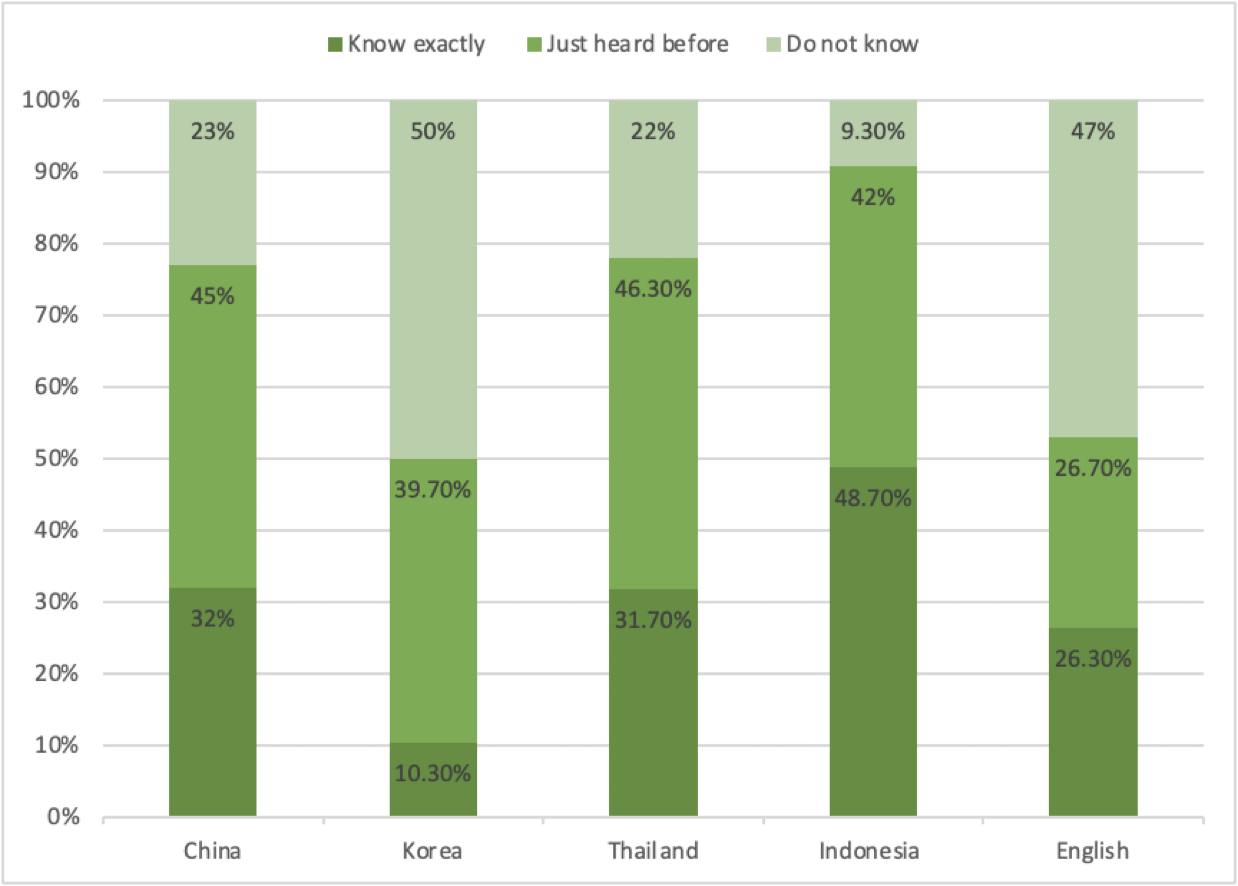
\includegraphics[width=0.8\linewidth]{Figure/Figure13.jpg}
  \centering
  \caption[Survey result of Q15]{Survey result of Q15(Do you know Safety tips or not ?)}
  \label{fig13}
\end{figure*}

\begin{figure*}[h]
  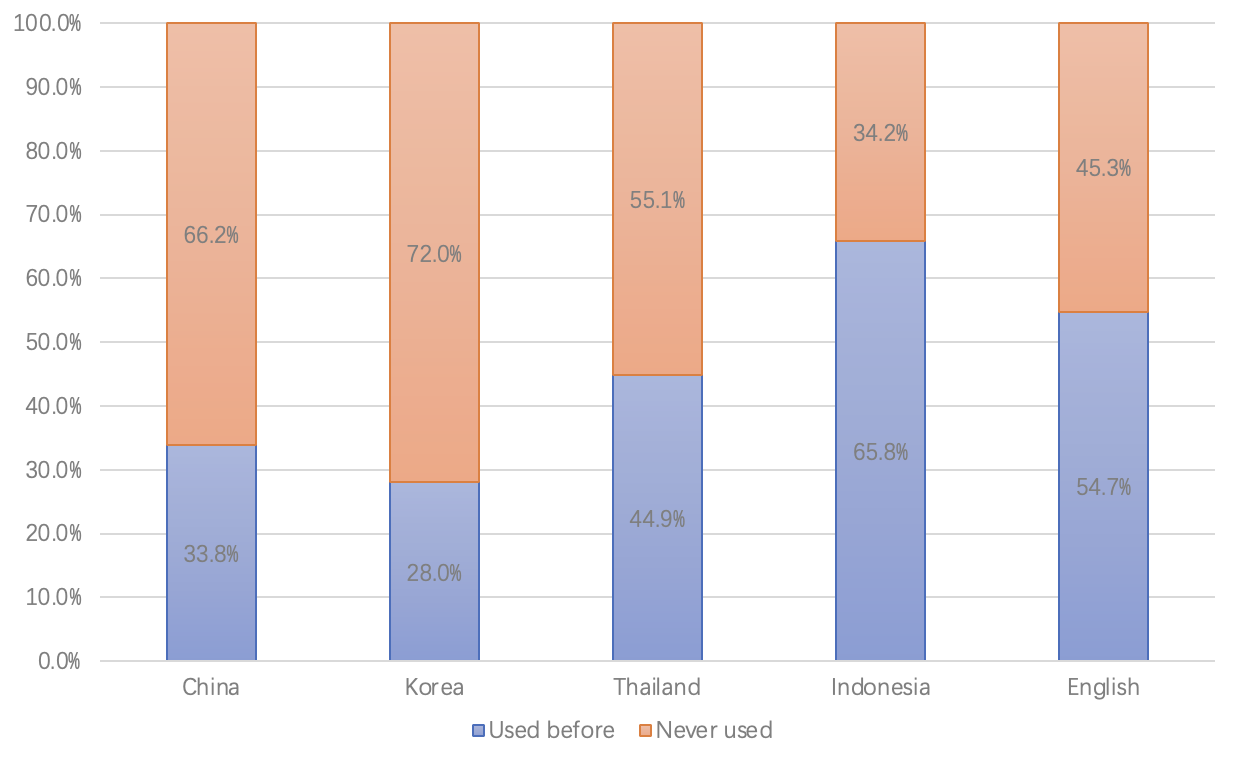
\includegraphics[width=0.8\linewidth]{Figure/Figure14.jpg}
  \centering
  \caption[Survey result of Q16]{Survey result of Q16(Do you use Safety tips before or not ?)}
  \label{fig14}
\end{figure*}

\begin{figure*}[h]
  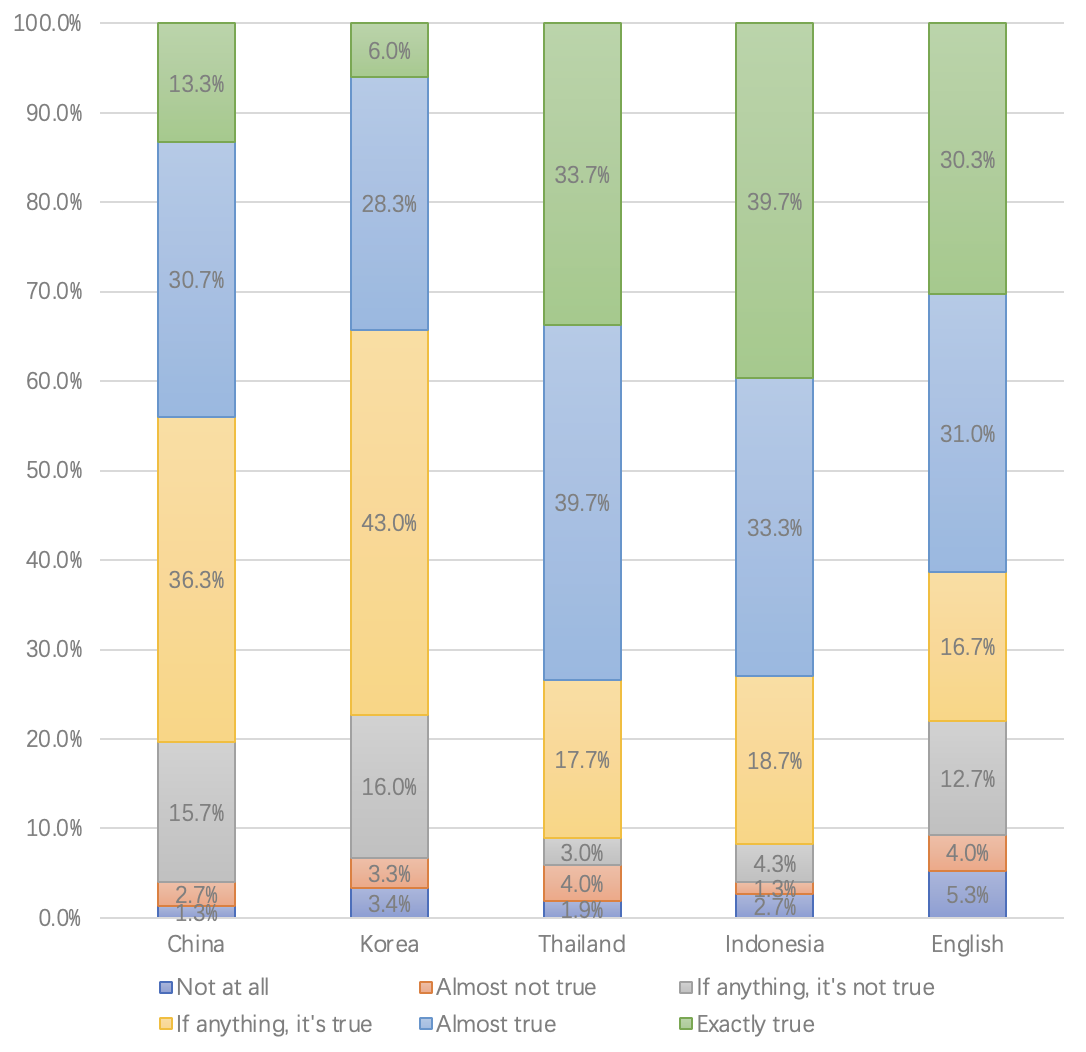
\includegraphics[width=0.8\linewidth]{Figure/Figure15.jpg}
  \centering
  \caption[Survey result of Q17\_1]{Survey result of Q17\_1(Will you trust Safety tips more than information from your own country ?)}
  \label{fig15}
\end{figure*}

\begin{figure*}[h]
  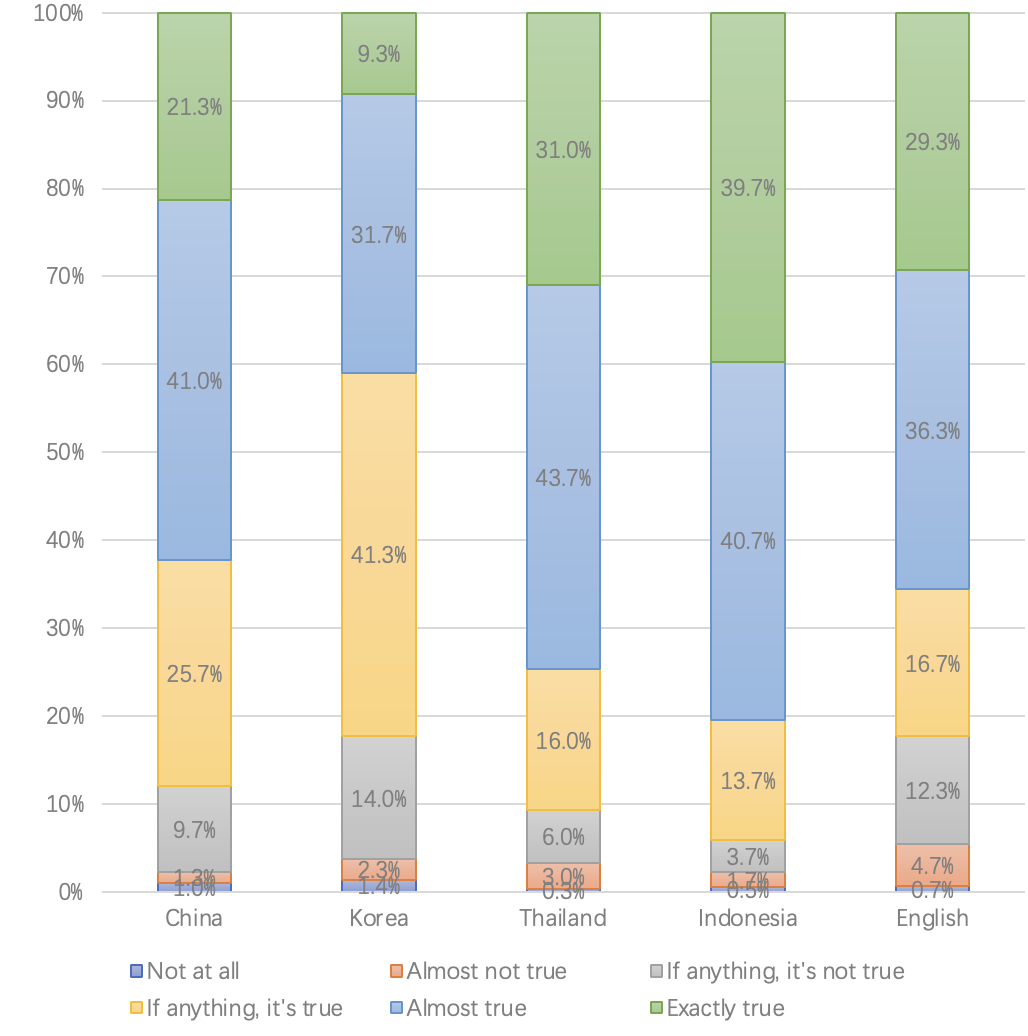
\includegraphics[width=0.8\linewidth]{Figure/Figure16.jpg}
  \centering
  \caption[Survey result of Q17\_2]{Survey result of Q17\_2(Will you use Safety tips before searching information from your own country ?)}
  \label{fig16}
\end{figure*}

\begin{figure*}[h]
  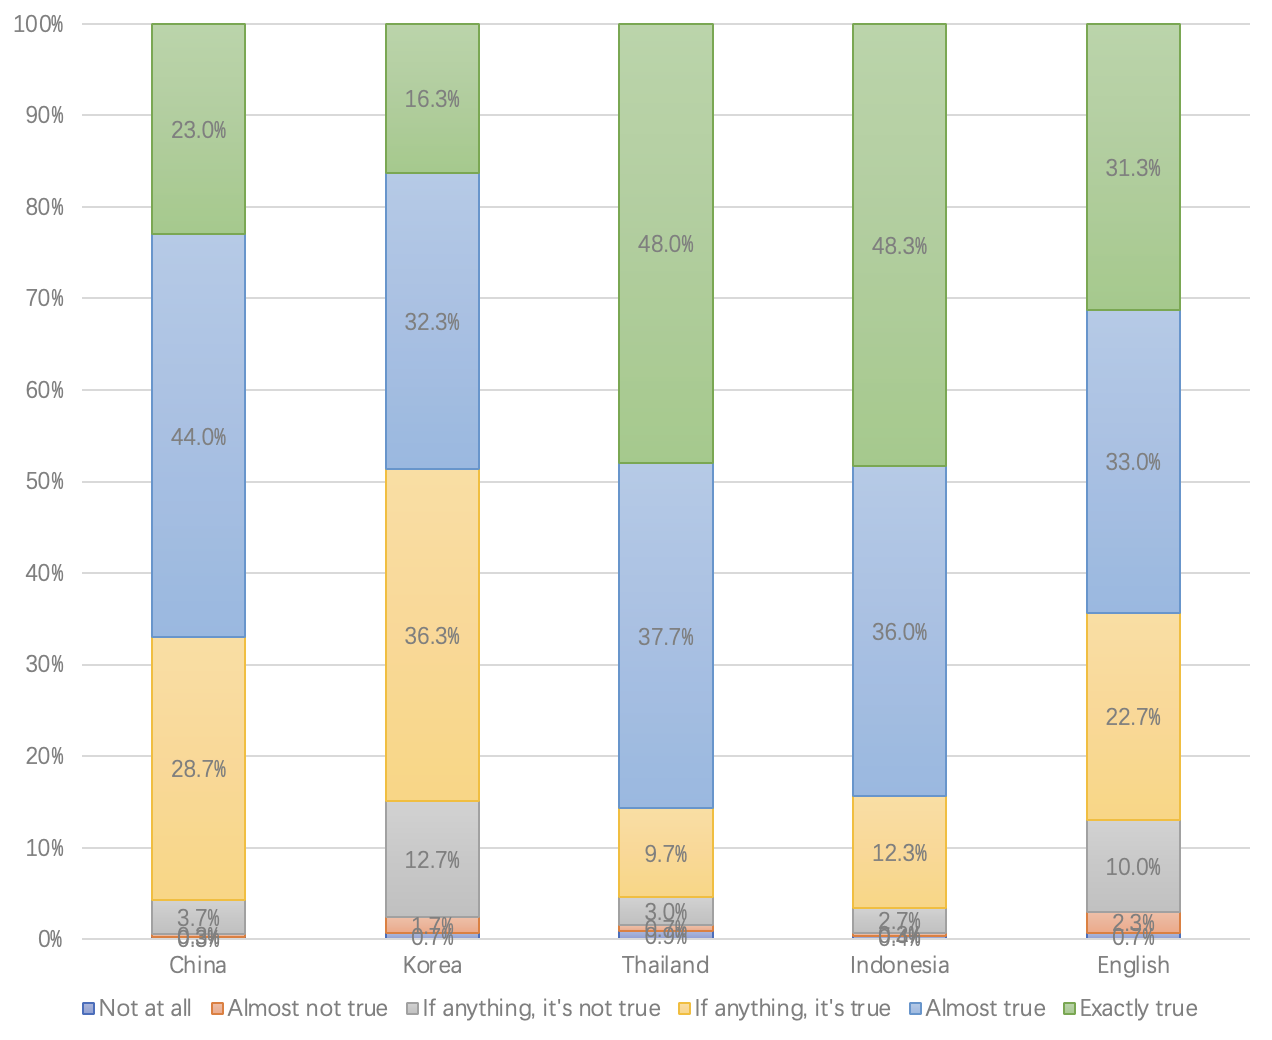
\includegraphics[width=0.8\linewidth]{Figure/Figure17.jpg}
  \centering
  \caption[Survey result of Q17\_3]{Survey result of Q17\_3(Do you think Safety tips could be useful during evacuation ?)}
  \label{fig17}
\end{figure*}

\begin{figure*}[h]
  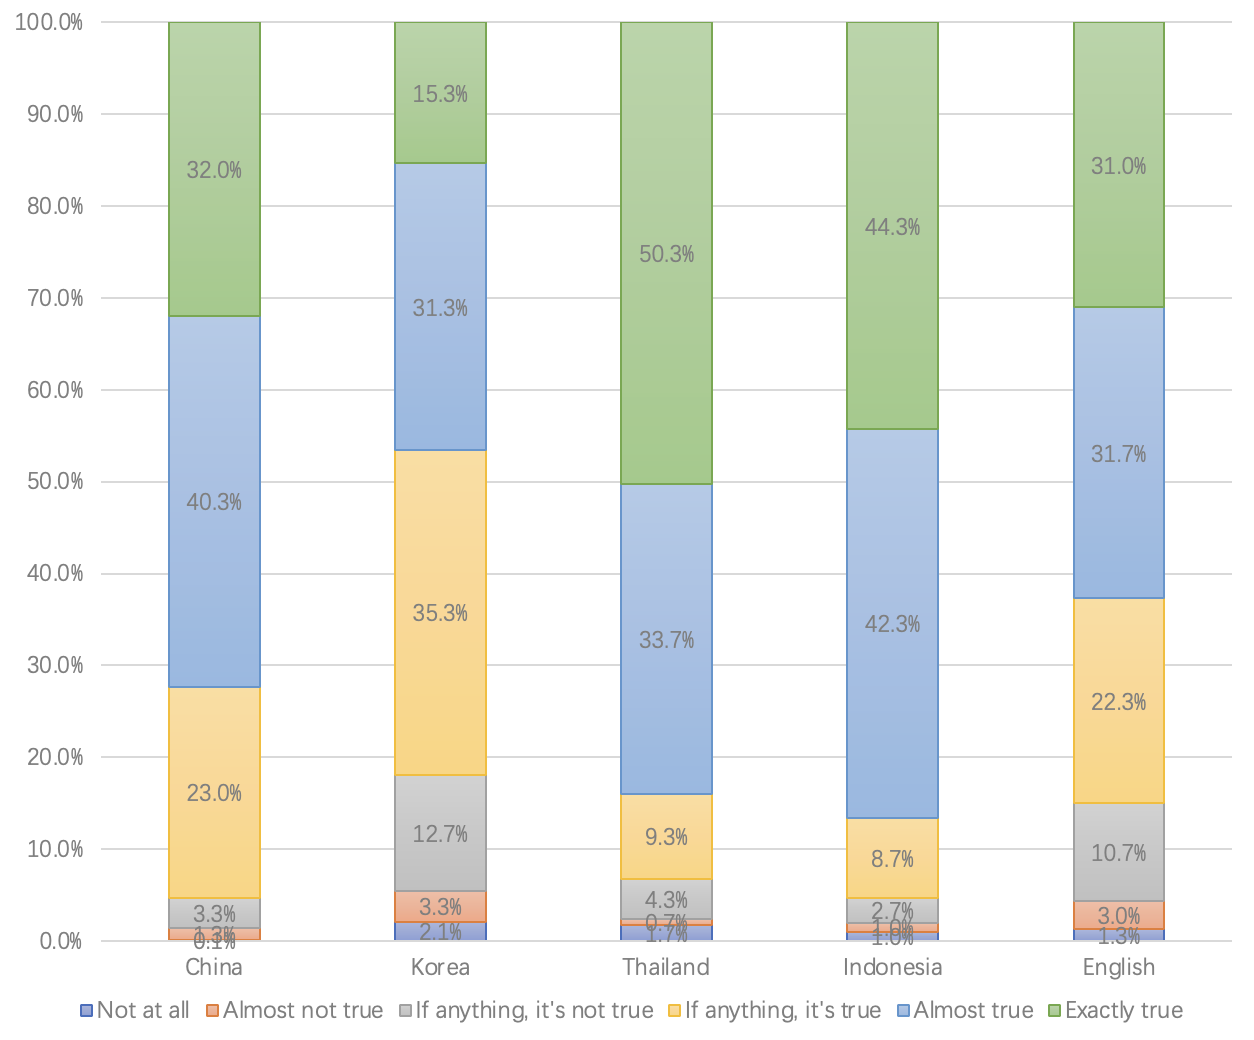
\includegraphics[width=0.8\linewidth]{Figure/Figure18.jpg}
  \centering
  \caption[Survey result of Q17\_4]{Survey result of Q17\_4(Will you use Safety tips in the future ?)}
  \label{fig18}
\end{figure*}

\begin{figure*}[h]
  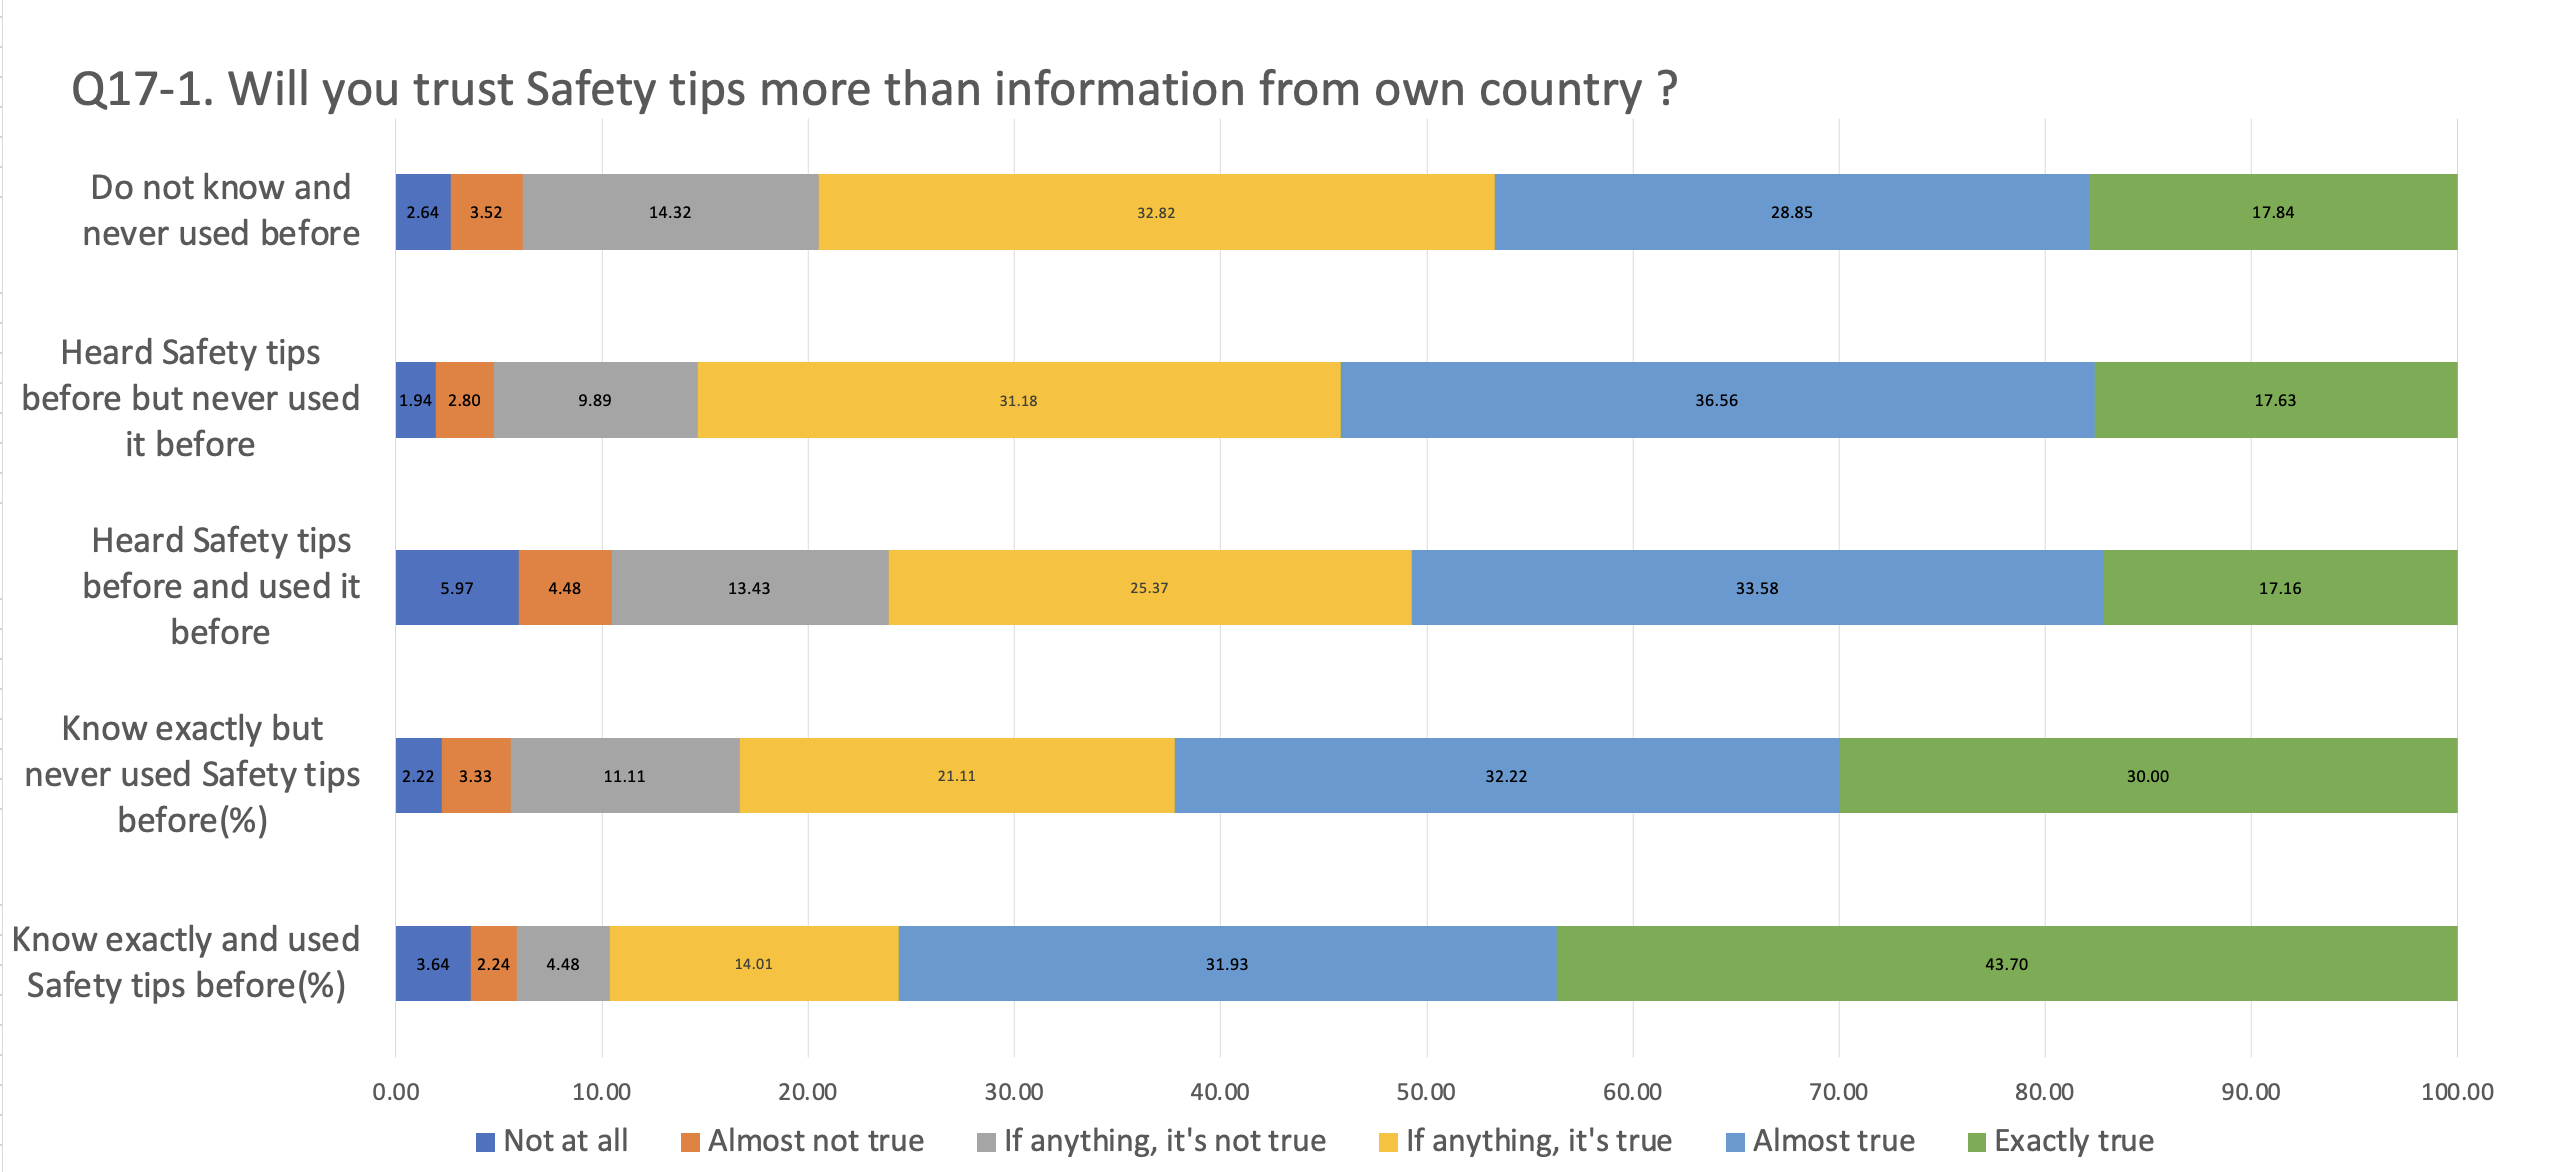
\includegraphics[width=0.8\linewidth]{Figure/Figure19.jpg}
  \centering
  \caption[5 groups of respondents' survey result of Q17\_1]{5 groups of respondents' survey result of Q17\_1(Will you trust Safety tips more than information from your own country ?)}
  \label{fig19}
\end{figure*}

\begin{figure*}[h]
  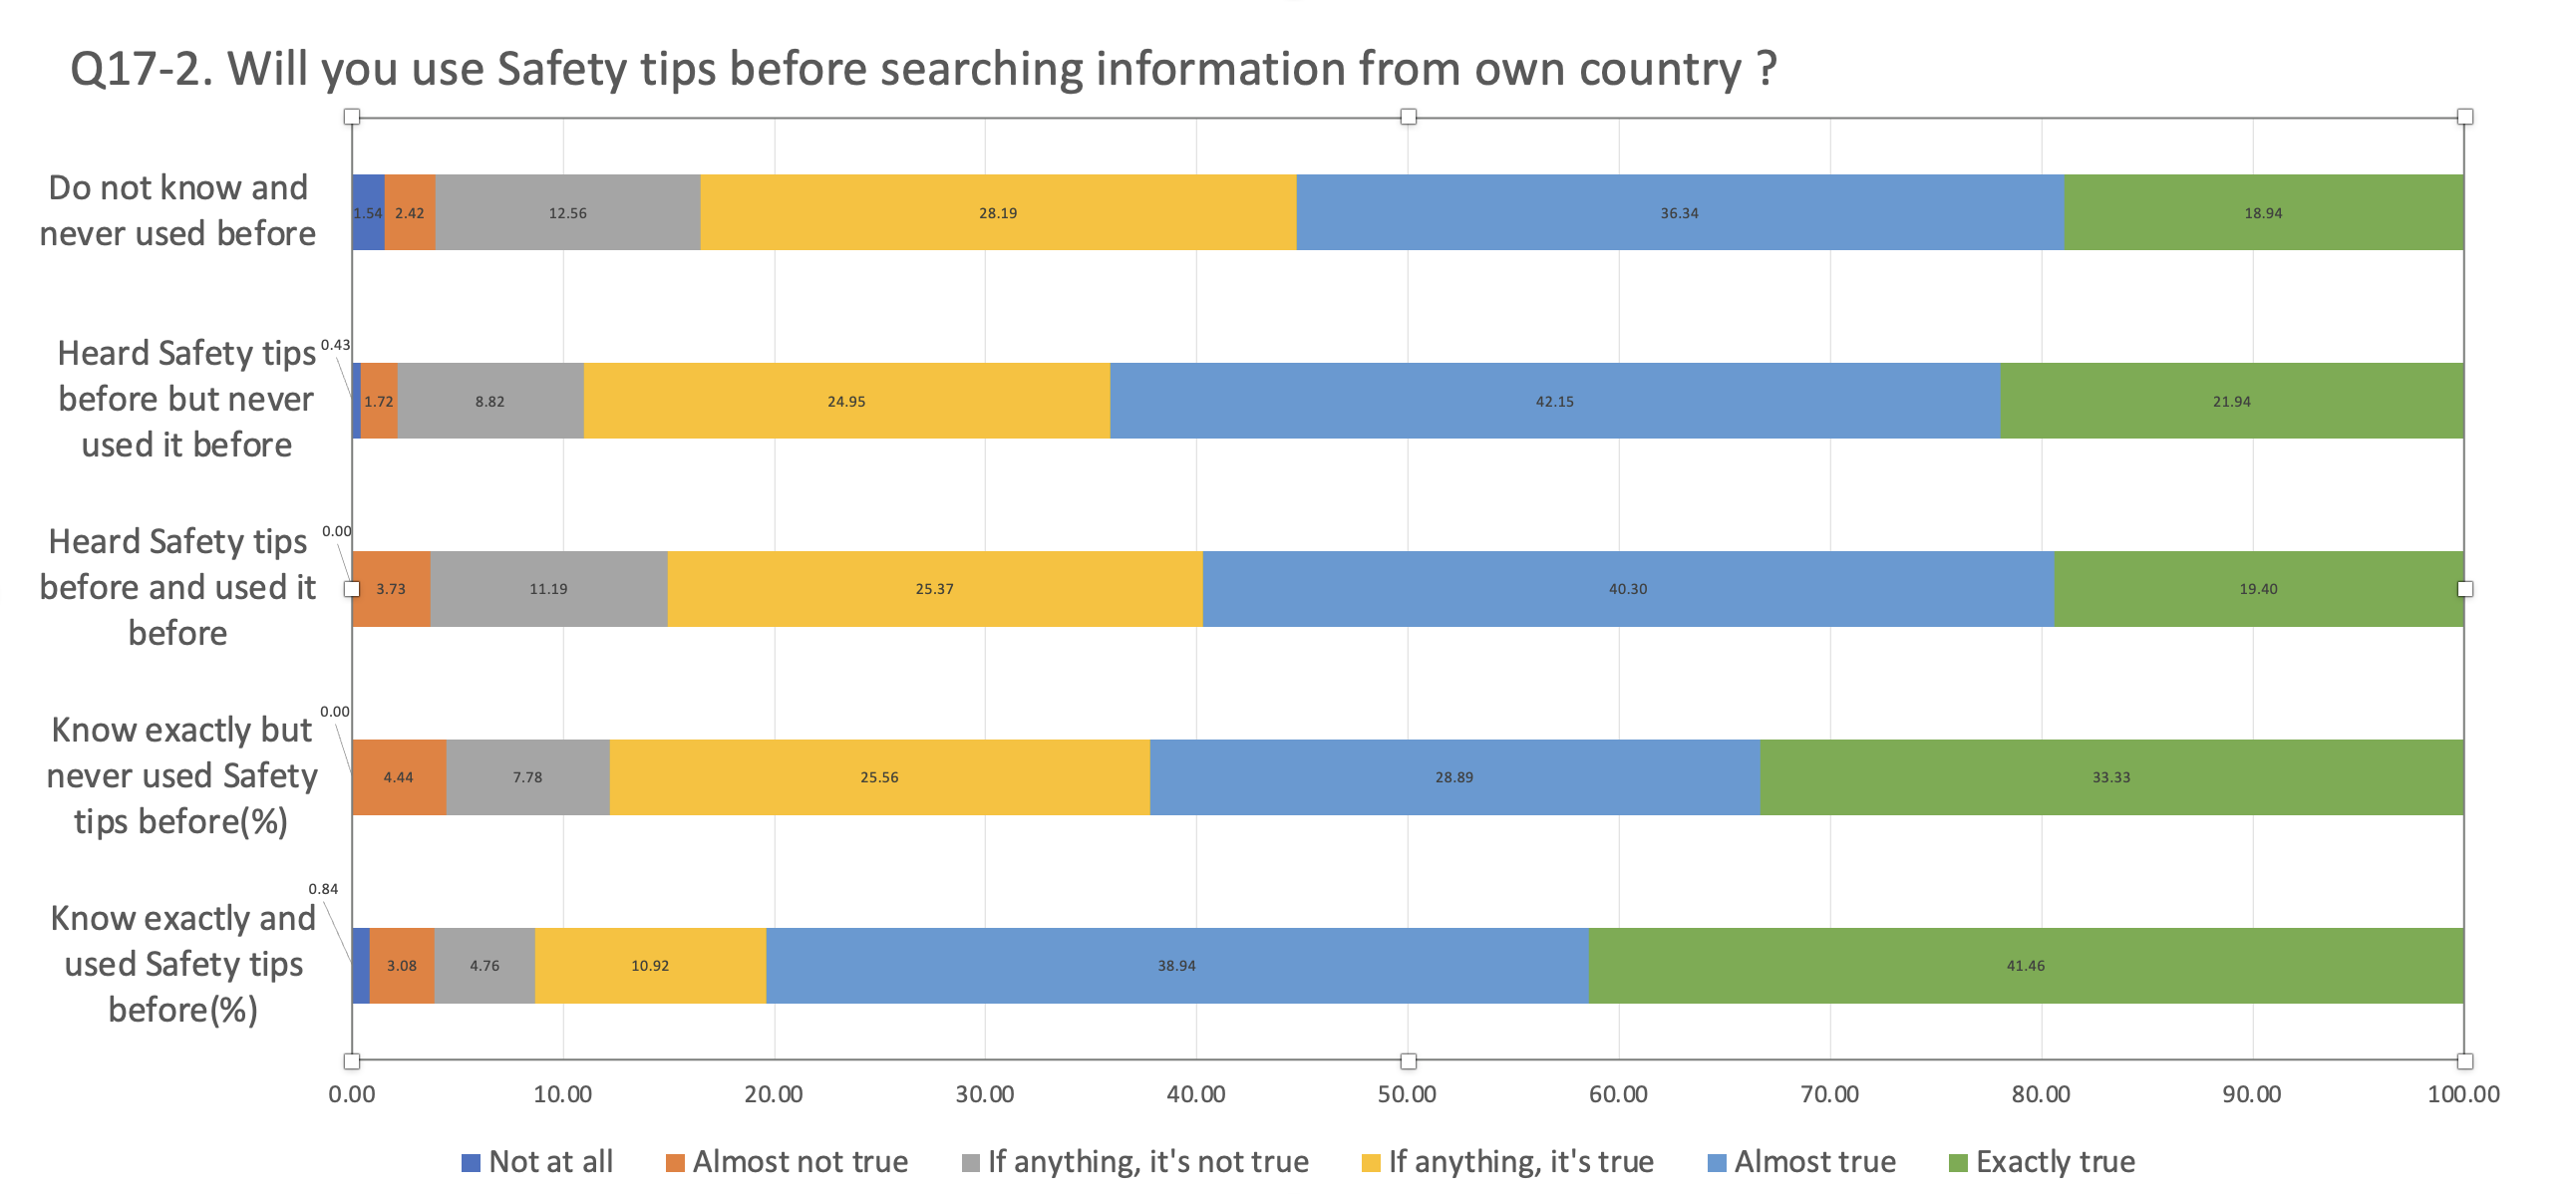
\includegraphics[width=0.8\linewidth]{Figure/Figure20.jpg}
  \centering
  \caption[5 groups of respondents' survey result of Q17\_2]{5 groups of respondents' survey result of Q17\_2(Will you use Safety tips before searching information from your own country ?)}
  \label{fig20}
\end{figure*}

\begin{figure*}[h]
  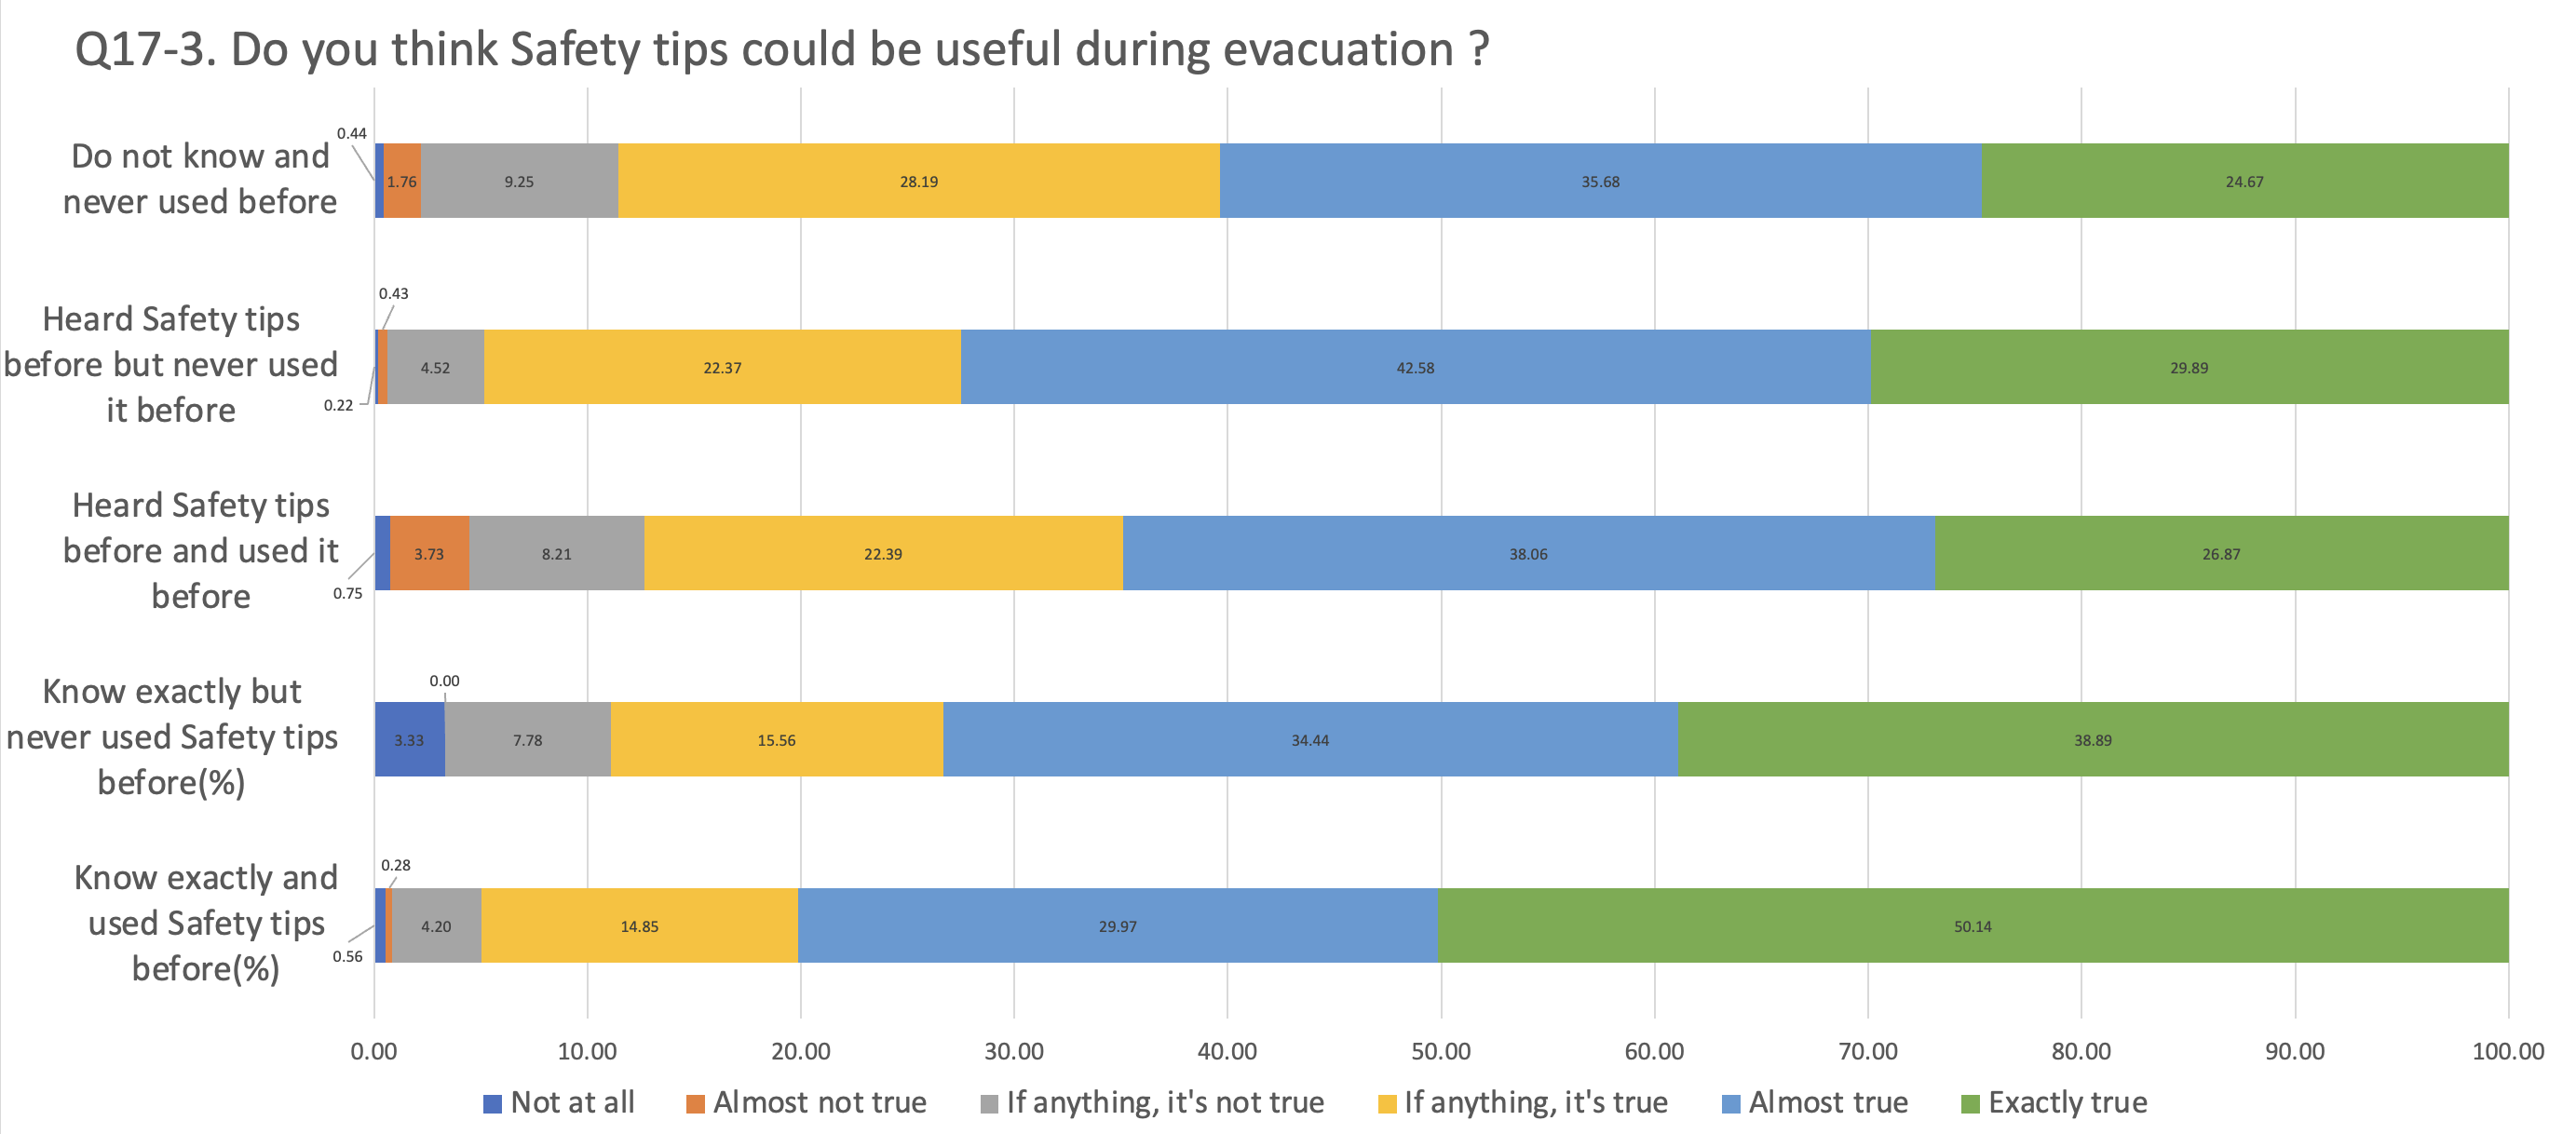
\includegraphics[width=0.8\linewidth]{Figure/Figure21.jpg}
  \centering
  \caption[5 groups of respondents' survey result of Q17\_3]{5 groups of respondents' survey result of Q17\_3(Do you think Safety tips could be useful during evacuation ?)}
  \label{fig21}
\end{figure*}

\begin{figure*}[h]
  \includegraphics[width=0.8\linewidth]{Figure/Figure22.jpg}
  \centering
  \caption[5 groups of respondents' survey result of Q17\_4]{5 groups of respondents' survey result of Q17\_4(Will you use Safety tips in the future ?)}
  \label{fig22}
\end{figure*}
%\fi

From the above results, we can conclude that from the usage experience, Safety Tips could be more popular and well-known in Indonesia(90\%), China(77\%), and Thailand(79\%) rather than in the UK(53\%) and Korea(50\%). Also, among those respondents that know Safety Tips or heard them before, their usage rate is lower than 70\%. China(33.8\%), Korea(28\%), Thailand(44.9\%), Indonesia(65.8\%) and the UK(54.7\%). 

Then from the attitude toward Safety Tips, we can conclude that over 77\% of the respondents say that they trust Safety Tips more than information from their own countries, over 82\% of the respondents say that they will use Safety tips to search information before from their own countries, and over 84\% of the respondents say that they believe Safety tips could be useful during evacuation and will use Safety tips in the future.

\subsection{Second Task}
In the second task, we aim to find whether the two factors of respondents' past awareness and whether they used it before had an impact on their attitudes toward Safety Tips. After dividing all respondents into 5 groups, we can find the differences between groups. 

For Q17\_1, Will the respondents trust Safety tips more than information from their country, the result shows in Figure~\ref{fig19}. we can find that respondents who "Know exactly and used Safety tips before" show the highest trust toward Safety Tips, as more than 75\% of the respondents said they trust the information on Safety Tips rather than from their own countries. Respondents who "Know exactly but never used Safety tips before" and "Heard Safety tips before but never used it before" are more likely to trust the information on Safety Tips. Respondents who "Heard Safety tips before and used it before" and "Do not know and never used before" show a relatively negative attitude on Safety Tips. 

For Q17\_2, Will the respondents use Safety tips before searching information from their country, the result shows in Figure~\ref{fig20}. we can find that the respondents who "Know exactly and used Safety tips before" show the highest usage possibility on Safety Tips, as more than 80\% of the respondents said Safety Tips have a higher priority of usage rather than from their own countries. Respondents that ‘Know exactly but never used Safety tips before' and ‘Heard Safety tips before but never used it before' show similar attitudes on the priority of using Safety Tips. Respondents that ‘Do not know and never used before' and ‘‘Heard Safety tips before and used it before' show a little bit lower usage priority. 

For Q17\_3, do the respondents think Safety tips could be useful during the evacuation, the result is shown in Figure~\ref{fig21}. we can find that respondents that "Know exactly and used Safety tips before" and "Heard Safety tips before but never used it before" show believe Safety Tips could be useful during evacuation. Respondents that "Do not know and never used before", "Heard Safety tips before and used it before", and "Know exactly but never used it before" are more likely to show lower usefulness of Safety Tips. 

For Q17\_4, will the respondents use Safety tips in the future, the result shows in Figure~\ref{fig22}. we can find that respondents that "Know exactly and used Safety tips before" and "Heard Safety tips before but never used it before" show higher usage possibly Safety Tips in the future. Respondents that "Do not know and never used before", "Heard Safety tips before and used it before", and "Know exactly but never used it before" show relatively lower usage possibility.

From the above results, we can conclude that respondents that "Know exactly and used Safety tips before" show higher trust and higher priority of use on Safety Tips, also they are more likely to believe Safety Tips can be useful during the evacuation, and they will use it in the future. And, respondents that "Heard Safety tips before but never used it before" show better attitude on Safety Tips rather than respondents that "Do not know and never used before", "Heard Safety tips before and used it before", and "Know exactly but never used it before".

\subsection{Third Task}

The third task is an independent sample T-test analysis, to test whether respondents' past awareness and usage experience of Safety Tips can significantly influence their attitudes towards Safety Tips. 

The T-test of respondents' gender is shown in Table~\ref{table24}. From the result, we can know that there has no significant difference in attitude(trust level, priority of use, Possibility of future use) toward Safety Tips between males and females. Only in the usefulness part, it shows that there has a significant difference. 

The T-test of respondents' age is shown in Table~\ref{table25}. From the result, we can know that there has a significant difference in attitude toward Safety Tips between respondents under age 40 and age over 40. 

The T-test of respondents' Japanese Level is shown in Table~\ref{table26}. From the result, we can know that there has a significant difference in attitude (trust level, priority of use) toward Safety Tips between respondents who can understand Japanese or not. But in the usefulness and Possibility of future use part, it shows that there has no significant difference. 


The T-test of respondents' previous awareness is shown in Table~\ref{table6}. We can deduce from the results that there is a significant difference in attitude toward Safety Tips between those who knew them and those who didn't. Those who have known of it before have a higher level of trust in Safety Tips and will prioritize using Safety Tips over information from their own countries. They also believe that this application could be useful during the evacuation and they have a higher possibility of use in the future. 

%%%%%%%%%%%%%%%%%%%
%\iffalse
\begin{table}[h]
\caption{T-test result: Gender with attitudes towards Safety Tips.}
\label{table24}
\centering
\begin{tabular}{|c|c|c|c|c|}
\hline
& \begin{tabular}{c}Male($=$1)\\(n=750)\end{tabular} & \begin{tabular}{c}Female($=$2)\\(n=750)\end{tabular} & t & p \\
\hline
Q17 Safetytips\_trust\_1 & 4.54$\pm$1.22 & 4.59$\pm$1.21 & $-$0.848 & 0.396 \\
\hline
Q17 Safetytips\_trust\_2 & 4.74$\pm$1.09 & 4.75$\pm$1.06 & $-$0.120 & 0.904 \\
\hline
Q17 Safetytips\_trust\_3 & 4.86$\pm$1.03 & 5.00$\pm$0.96 & $-$2.643 & 0.008 \\
\hline
Q17 Safetytips\_trust\_4 & 4.88$\pm$1.09 & 5.94$\pm$1.07 & $-$0.933 & 0.351 \\
\hline
\end{tabular}
\end{table}

\begin{table}[h]
\caption{T-test result: Age with attitudes towards Safety Tips.}
\label{table25}
\centering
\begin{tabular}{|c|c|c|c|c|}
\hline
& \begin{tabular}{c}Age under 39($<$4)\\(n=370)\end{tabular} & \begin{tabular}{c}Age over 40($>=$4)\\(n=1130)\end{tabular} & t & p \\
\hline
Q17 Safetytips\_trust\_1 & 4.34$\pm$1.30 & 4.64$\pm$1.18 & 4.015 & 0.000 \\
\hline
Q17 Safetytips\_trust\_2 & 4.57$\pm$1.14 & 4.80$\pm$1.05 & 3.361 & 0.001 \\
\hline
Q17 Safetytips\_trust\_3 & 4.78$\pm$1.05 & 4.98$\pm$0.98 & 3.204 & 0.001 \\
\hline
Q17 Safetytips\_trust\_4 & 4.78$\pm$1.38 & 4.95$\pm$1.06& 2.555 & 0.011 \\
\hline
\end{tabular}
\end{table}
%\fi

\begin{table}[h]
\caption{T-test result: Japanese Level with attitudes towards Safety Tips.}
\label{table26}
\centering
\begin{tabular}{|c|c|c|c|c|}
\hline
& \begin{tabular}{c}can understand\\($>=$3)(n=453)\end{tabular} & \begin{tabular}{c}can not understand\\($<$3)(n=1047)\end{tabular} & t & p \\
\hline
Q17 Safetytips\_trust\_1 & 4.73$\pm$1.22 & 4.49$\pm$1.21 & 3.455 & 0.001 \\
\hline
Q17 Safetytips\_trust\_2 & 4.83$\pm$1.08& 4.71$\pm$1.07 & 1.977 & 0.048 \\
\hline
Q17 Safetytips\_trust\_3 & 4.99$\pm$1.01 & 4.90 $\pm$0.99 & 1.537 & 0.125 \\
\hline
Q17 Safetytips\_trust\_4 & 4.99$\pm$1.05 & 4.88$\pm$1.09 & 1.841 & 0.066 \\
\hline
\end{tabular}
\end{table}


\begin{table}[h]
  \caption{T-test result: past awareness of Safety Tips with attitudes towards Safety Tips. }
  \label{table6}
  \centering
  \begin{tabular}{|c|c|c|c|c|}
  \hline
     & \begin{tabular}{c}Q15 Safety tips:\\don't know ($=$1)\\(n=454)\end{tabular} & \begin{tabular}{c}Q15 Safety tips:\\know($>=$2)\\(n=1046)\end{tabular} & t & p \\
  \hline
   Q17 Safetytips\_trust\_1 & 4.35$\pm$1.19 & 4.66$\pm$1.22 & 4.49 & 0.000 \\
  \hline
   Q17 Safetytips\_trust\_2 & 4.52$\pm$1.10 & 4.84$\pm$1.05 & 5.18 & 0.000 \\
  \hline
   Q17 Safetytips\_trust\_3 & 4.71$\pm$1.02 & 5.03$\pm$0.97 & 5.61 & 0.000 \\
  \hline
   Q17 Safetytips\_trust\_4 & 4.59$\pm$1.15 & 5.05$\pm$1.02 & 7.43 & 0.000 \\
  \hline
  \end{tabular}
\end{table}


The T-test of respondents' utilizing experience is shown in Table~\ref{table7}. The results show that there was no significant difference between the respondents' future use and whether they had used it before, but there was a significant difference between their attitude toward Safety Tips (trust level, priority of use, usefulness) and whether they had used safety tips before or not. Respondents who have used Safety Tips before have a higher level of trust in them and will prioritize Safety Tips over their own countries. They also believe that this application would come in useful during the evacuation.

%%%%%%%%%%%%%%%%%%%
%\iffalse
\begin{table}[h]
  \caption{T-test result: using experience of Safety Tips with attitudes towards Safety Tips.}
  \label{table7}
  \centering
  \begin{tabular}{|c|c|c|c|c|}
  \hline
     & \begin{tabular}{c}Q16 Safetytips\_use:\\used before($=$1)\\(n=491)\end{tabular} & \begin{tabular}{c}Q16 Safetytips\_use:\\never used before($=$0)\\(n=555)\end{tabular} & t & p \\
  \hline
   Q17 Safetytips\_trust\_1 & 4.80$\pm$1.31 & 4.53$\pm$1.12 & $-$3.49 & 0.001 \\
  \hline
   Q17 Safetytips\_trust\_2 & 4.95$\pm$1.08 & 4.74$\pm$1.01 & $-$3.38 & 0.001 \\
  \hline
   Q17 Safetytips\_trust\_3 & 5.10$\pm$1.01 & 4.96$\pm$0.94 & $-$2.34 & 0.019 \\
  \hline
   Q17 Safetytips\_trust\_4 & 5.11$\pm$1.02 & 5.00$\pm$1.01 & $-$1.72 & 0.086 \\
  \hline
  \end{tabular}
\end{table}
%\fi





\section{Results for Objective 2 }
\subsection{Model 1}

We constructed the SEM model 1 shown in Figure~\ref{fig23} based on the previous hypotheses in Chapter 4.2 to explore the relationship between the latent variables of "Training Experience", "Consciousness", "Knowledge", and "Attitudes toward Safety Tips". The five manifest variables of "Consciousness" (the responses of Q1-Q5), the two manifest variables of "Knowledge" (the responses of Q9-Q10), and the four manifest variables of  "Attitudes toward Safety Tips" (the responses of Q17\_1-Q17\_4) are all continuum selections, so it is necessary to test the score reliability coefficient. When multiple questions are asked about a characteristic and the sum of the responses (scale scores) is used as the characteristic scale, the reliability coefficient that assesses whether each questionnaire item (variable) measures the same concept or object as a whole (internal consistency) is called Cronbach's alpha. Cronbach's alpha is calculated by the following formula. 
\begin{equation}
\alpha = \frac{m}{m-1} \left(1 - \frac{\displaystyle \sum_{i = 1}^m{{\sigma_i}^2}}{{\sigma_x}^2} \right)
\end{equation}
$m$ means the number of items in the question; ${\sigma_i}^2$ means the variance of each question item; ${\sigma_x}^2$ means the variance of the total scale score for each question item. Cronbach's alpha has a value between 0 and 1, and the closer the value is to 1, the more reliable it is. The evaluation of Cronbach's alpha, as shown in Figure~\ref{fig24}, was suggested by George and Mallery~\cite{ref1}. Cronbach's alpha  Cronbach's alpha of 0.9 indicates excellent internal consistency, 0.8 indicates good, 0.7 indicates acceptable, 0.6 indicates poor, and 0.5 unacceptable. The results of the alpha reliability coefficient test are shown in Table~\ref{table8}, the Cronbach's alpha values of Q1-Q5 is 0.869, for Q9-Q10 is 0.927, and for Q7\_1-Q17\_4 is 0.871. The total Cronbach's alpha value for all the above variables is 0.935. We can find that the Cronbach's alpha value of any one of them is satisfying the evaluation criteria.

%%%%%%%%%%%%%%%%%%%
%\iffalse
\begin{figure*}[h]
  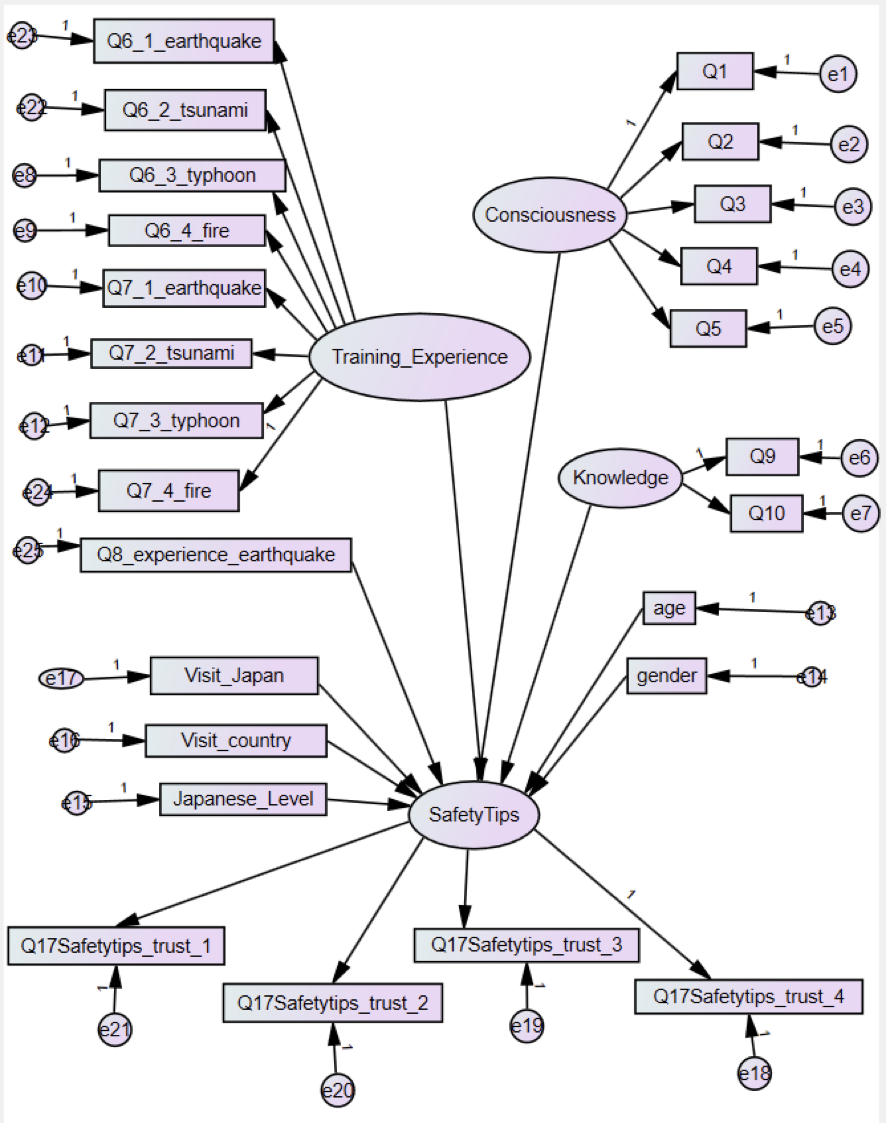
\includegraphics[width=0.5\linewidth]{Figure/Figure23.jpg}
  \centering
  \caption{SEM model 1}
  \label{fig23}
\end{figure*}

\begin{figure*}[h]
  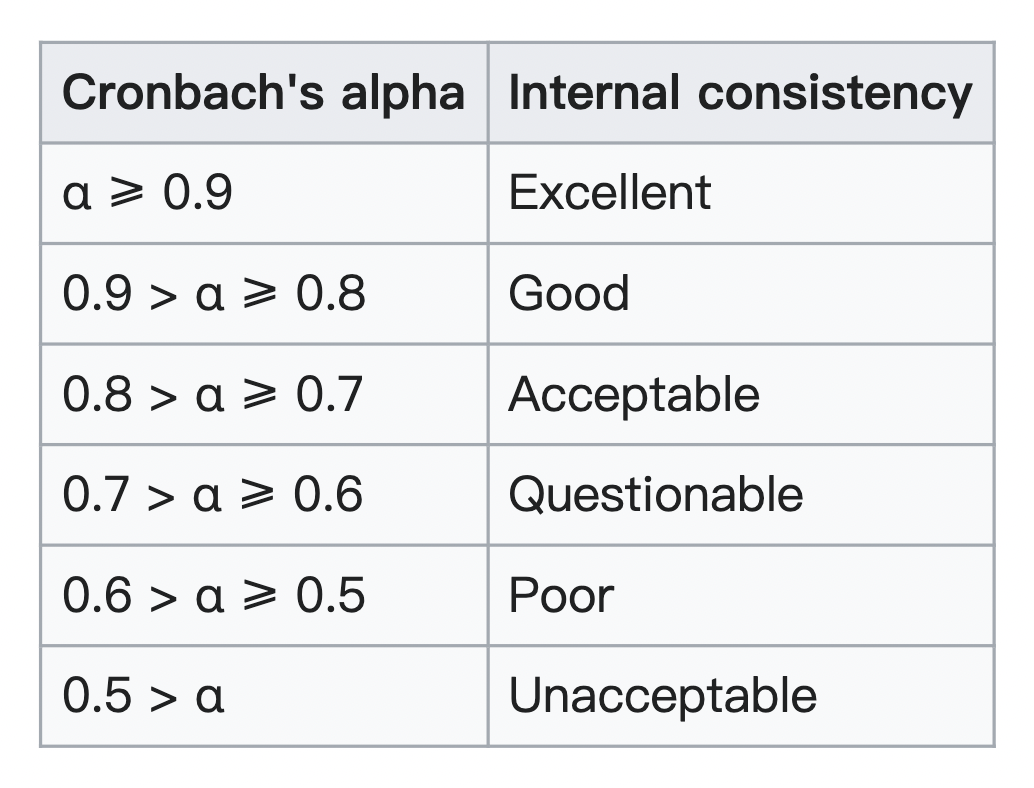
\includegraphics[width=0.5\linewidth]{Figure/Figure24.jpg}
  \centering
  \caption{Evaluation of score reliability coefficient test}
  \label{fig24}
\end{figure*}


\begin{table}[h]
  \caption{Result of score reliability coefficient test}
  \label{table8}
  \centering
  \begin{tabular}{|c|c|c|}
  \hline
          & Cronbach's alpha value & Objects \\
 \hline 
  Q1 to Q5 & 0.869 & 20 \\
 \hline
  Q9 and Q10 & 0.927 & 15 \\
 \hline 
  Q17 & 0.871 & 4 \\
 \hline
  All & 0.935 & 39 \\
 \hline
  \end{tabular}
\end{table}
%\fi

The result of Regression Weights for Model 1 shows in Table~\ref{table9} and the result of Standard Regression Weights for Model 1 is shown in Table~\ref{table10}. From the result, we can find that "Consciousness", "Knowledge", "Earthquake experience", "Japanese level" could show significant relationships with respondents' attitude on Safety Tips. While, "Age", "Gender", "Visit Japan", "Visit country" don't show significant relationships with respondents' attitudes toward Safety Tips. Currently, "training experience" also doesn't have a significant relationship with respondents' attitude on Safety Tips. Because "training experience" is a potential variable in our original hypothesis, I'd like to go deeper into the relationship with some improvements. We can get a better estimate of the true correlation by disattenuated the variables, according to D. Streiner~\cite{Streiner2006BuildingAB}. Two things happen when we add extra variables. First, the model's ability to account for more variance grows. Each new variable, on the other hand, enhances the error variance. As a result, the previous model will struggle to accommodate the additional data, which is a consequence of adding more variables to the model. We can see that Q6 1/2/3/4 and Q7 1/2/3/4 both have a significant relationship with "Training Experience" based on the results of Table~\ref{table9} Regression Weights. However, the estimated value of Q7 1/2/3/4 is much lower than the estimated value of Q6 1/2/3/4, as seen in Table~\ref{table10} Standardized Regression Weights. This means that Q6 is better than Q7 at expressing the latent variable "Training Experience". The two manifest variables are similar in structure: Q6 is for the experience of a given event, and the total score is used as data, whereas Q7 is for the number of times. Because the similarity of the two variables causes a significant amount of inaccuracy in the expression of the latent variable, we'll delete Q7 and keep only Q6 as the manifest variable to express "Training experience" as a way to improve the model. Furthermore, we believe there may have a correlation relationship between "Training Experience", "Consciousness", and "Knowledge". Therefore adding the correlation between these three latent variables is another way to improve the model. Finally, since the result shows that "Age", "Gender", "Visit Japan", and "Visit Country" have no significant relationship with "Attitude toward Safety Tips", deleting these four variables could be also a way to improve the model. Based on the above three improvement ideas shown on the left side of  Figure~\ref{fig25}, we construct Model 2 shown on the right side of Figure~\ref{fig25}.

%%%%%%%%%%%%%%%%%%%
%\iffalse
\begin{figure*}[h]
  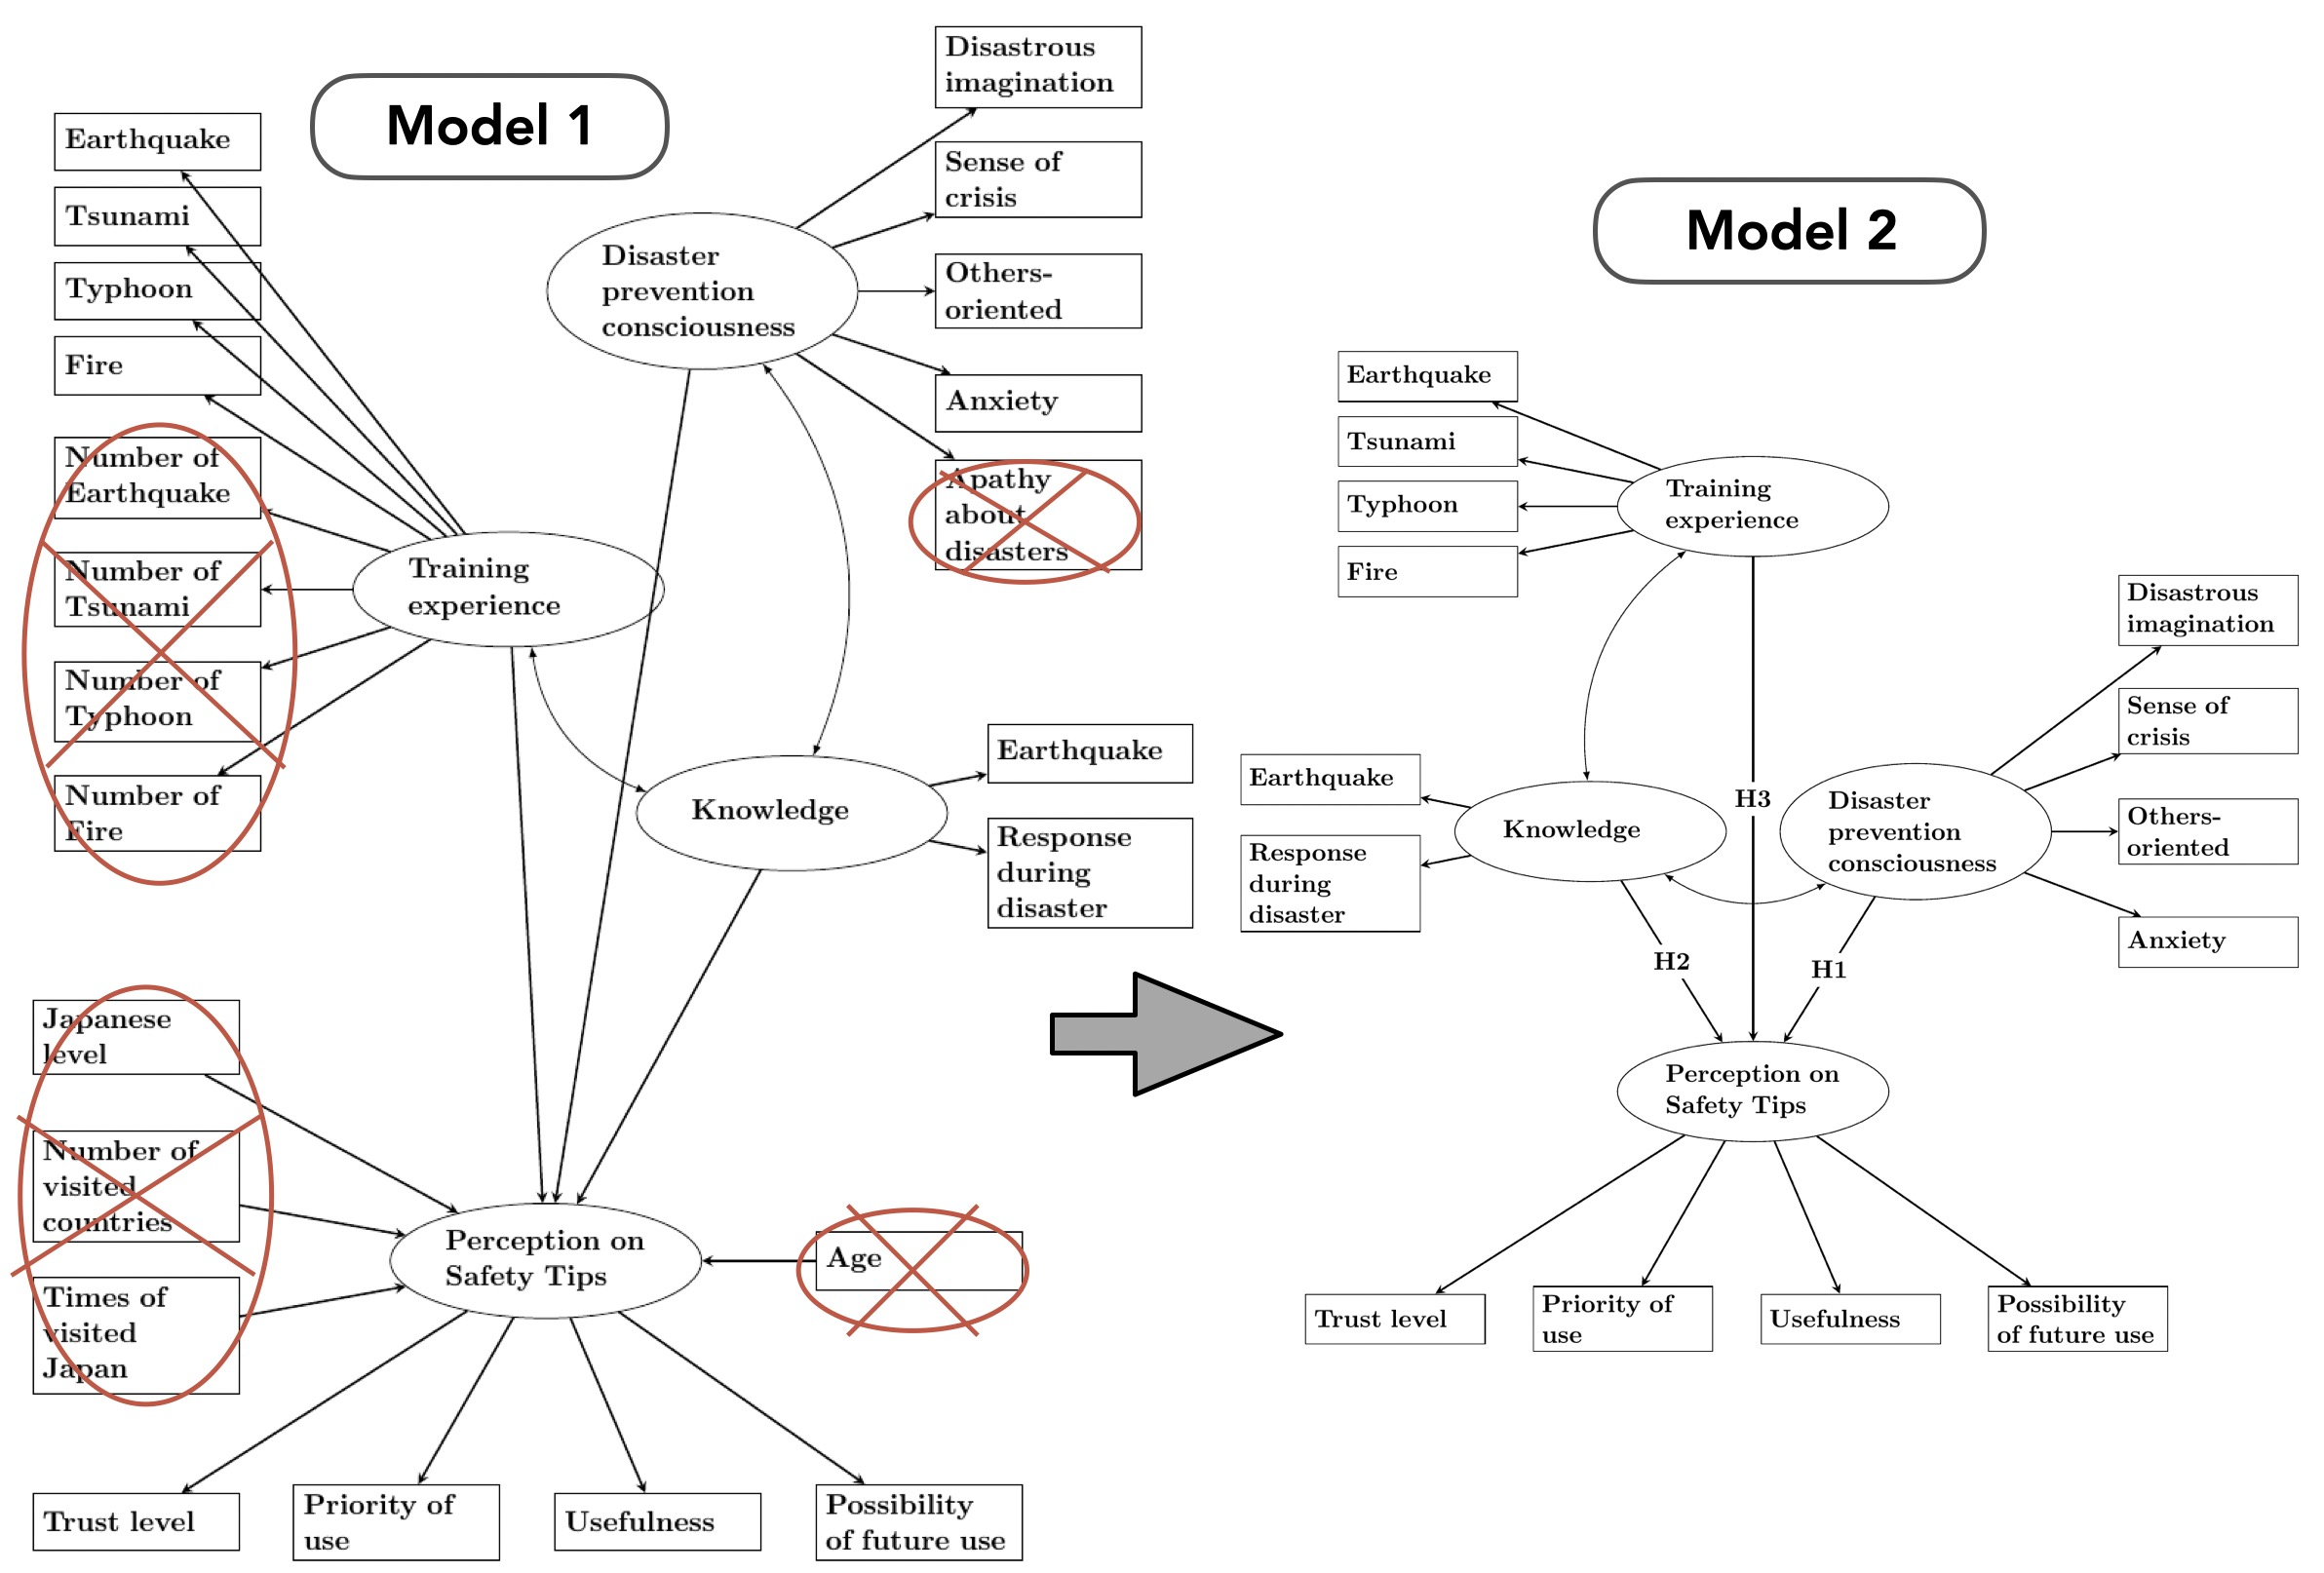
\includegraphics[width=\linewidth]{Figure/Figure25.png}
  \centering
  \caption[SEM model 2]{Left side: the diagram contains the improvement points made based on Model 1,Right side: Model 2}
  \label{fig25}
\end{figure*}


\begin{table}[h]
  \caption{Regression Weights of Model 1}
  \label{table9}
  \centering
  \begin{tabular}{|l|c|l|c|c|}
 \hline
 \multicolumn{3}{|c|}{Regression Weights} & Estimate & p \\
 \hline
  Safety Tips & $\longleftarrow$ & Age & 0.036 & 0.007 \\ 
  Safety Tips & $\longleftarrow$ & Gender &0.065 & 0.053 \\
  Safety Tips & $\longleftarrow$ & Training Experience & $-$0.075 & 0.003 \\
  Safety Tips & $\longleftarrow$ & Consciousness & 0.194 & *** \\
  Safety Tips & $\longleftarrow$ & Knowledge & 1.448 & *** \\
  Safety Tips & $\longleftarrow$ & Visit Country & 0.002 & 0.803 \\
  Safety Tips & $\longleftarrow$ & Japanese Level & $-$0.095 & *** \\
  Safety Tips & $\longleftarrow$ & Visit Japan & 0.006 & 0.377 \\
  Safety Tips & $\longleftarrow$ & Q8\_experience\_earthquake & $-$0.225 & *** \\
  Q1              & $\longleftarrow$ & Consciousness & 1.000 &  \\
  Q2              & $\longleftarrow$ & Consciousness & 0.790 & *** \\
  Q3              & $\longleftarrow$ & Consciousness & 0.868 & *** \\
  Q4              & $\longleftarrow$ & Consciousness & 0.677 & *** \\
  Q5              & $\longleftarrow$ & Consciousness & 0.158 & *** \\
  Q6\_1\_earthquake & $\longleftarrow$ & Training Experience & 3.677 & *** \\
  Q6\_2\_tsunami & $\longleftarrow$ & Training Experience & 3.341 & *** \\
  Q6\_3\_typhoon & $\longleftarrow$ & Training Experience & 3.576 & *** \\
  Q6\_4\_fire & $\longleftarrow$ & Training Experience & 3.672 & *** \\
  Q7\_1\_earthquake & $\longleftarrow$ & Training Experience & 0.949 & *** \\
  Q7\_2\_tsunami & $\longleftarrow$ & Training Experience & 0.614 & *** \\
  Q7\_3\_typhoon & $\longleftarrow$ & Training Experience & 0.725 & *** \\
  Q7\_4\_fire & $\longleftarrow$ & Training Experience & 1.000 & \\
  Q9             & $\longleftarrow$ & Knowledge & 1.000 & \\
  Q10           & $\longleftarrow$ & Knowledge & 1.028 & *** \\
  Q17 Safetytips\_trust\_1 & $\longleftarrow$ & Safety Tips & 1.118 & *** \\
  Q17 Safetytips\_trust\_2 & $\longleftarrow$ & Safety Tips & 1.000 & \\
  Q17 Safetytips\_trust\_3 & $\longleftarrow$ & Safety Tips & 1.012 & *** \\
  Q17 Safetytips\_trust\_4 & $\longleftarrow$ & Safety Tips & 1.000 & \\
 \hline
  \end{tabular}
\end{table}

\begin{table}[h]
  \caption{Standardized Regression Weights of Model 1 }
  \label{table10}
  \centering
  \begin{tabular}{|l|c|l|c|}
 \hline
 \multicolumn{3}{|c|}{Standardized Regression Weights} & Estimate \\
 \hline
  Safety Tips & $\longleftarrow$ & Age & 0.057 \\ 
  Safety Tips & $\longleftarrow$ & Gender &0.040 \\
  Safety Tips & $\longleftarrow$ & Training Experience & $-$0.067 \\
  Safety Tips & $\longleftarrow$ & Consciousness & 0.191 \\
  Safety Tips & $\longleftarrow$ & Knowledge & 0.967 \\
  Safety Tips & $\longleftarrow$ & Visit Country & 0.005 \\
  Safety Tips & $\longleftarrow$ & Japanese Level & $-$0.094 \\
  Safety Tips & $\longleftarrow$ & Visit Japan & 0.018 \\
  Safety Tips & $\longleftarrow$ & Q8\_experience\_earthquake & $-$0.102 \\
  Q1              & $\longleftarrow$ & Consciousness & 0.760\\
  Q2              & $\longleftarrow$ & Consciousness & 0.706 \\
  Q3              & $\longleftarrow$ & Consciousness & 0.703\\
  Q4              & $\longleftarrow$ & Consciousness & 0.540 \\
  Q5              & $\longleftarrow$ & Consciousness & 0.112 \\
  Q6\_1\_earthquake & $\longleftarrow$ & Training Experience & 0.785 \\
  Q6\_2\_tsunami & $\longleftarrow$ & Training Experience & 0.838 \\
  Q6\_3\_typhoon & $\longleftarrow$ & Training Experience & 0.862 \\
  Q6\_4\_fire & $\longleftarrow$ & Training Experience & 0.706 \\
  Q7\_1\_earthquake & $\longleftarrow$ & Training Experience & 0.484 \\
  Q7\_2\_tsunami & $\longleftarrow$ & Training Experience & 0.473 \\
  Q7\_3\_typhoon & $\longleftarrow$ & Training Experience & 0.521 \\
  Q7\_4\_fire & $\longleftarrow$ & Training Experience & 0.465\\
  Q9             & $\longleftarrow$ & Knowledge & 0.512\\
  Q10           & $\longleftarrow$ & Knowledge & 0.600 \\
  Q17 Safetytips\_trust\_1 & $\longleftarrow$ & Safety Tips & 0.757 \\
  Q17 Safetytips\_trust\_2 & $\longleftarrow$ & Safety Tips & 0.773 \\
  Q17 Safetytips\_trust\_3 & $\longleftarrow$ & Safety Tips & 0.829 \\
  Q17 Safetytips\_trust\_4 & $\longleftarrow$ & Safety Tips & 0.760 \\
 \hline
  \end{tabular}
\end{table}
%\fi

\subsection{Model 2}

The result of Regression Weights for Model 2 shows in Table~\ref{table11}. From the result, we can find that "Consciousness", "Knowledge", "Earthquake experience", "Training Experience", and "Japanese level" could all show significant relationships with respondents" attitude toward Safety Tips. Then, the result of Standard Regression Weights for Model 1 shows in Table~\ref{table12}. From the result, we can find that "Consciousness", "Earthquake experience", "Training Experience", and "Japanese level" could be negatively related to respondents" attitudes towards Safety Tips, as the estimated values are negative numbers. While "Knowledge" could be positively related to respondents" attitudes towards Safety Tips, as the estimated value is 3.068. From the  Regression Weights, we can find that the p-value of Q5 and Consciousness is 0.034, which means Q5 is not significant enough to express Consciousness, so to improve the model, Model 3 will delete Q5, only use Q1 to Q4 to express latent variable "Consciousness". The result of the correlation relationship between "Consciousness", "Knowledge", "Training Experience" was shown in Table~\ref{table13} and Table~\ref{table14}. The result confirmed that "Consciousness", "Knowledge", "Training Experience" could be all positively correlated with each other. Among them, "Consciousness" and "Knowledge" show the highest correlation. 

%%%%%%%%%%%%%%%%%%%
%\iffalse
\begin{table}[h]
  \caption{Regression Weights of Model 2}
  \label{table11}
  \centering
  \begin{tabular}{|l|c|l|c|c|}
 \hline
 \multicolumn{3}{|c|}{Regression Weights} & Estimate & p \\
 \hline
  Safety Tips & $\longleftarrow$ & Training Experience & $-$0.146 & *** \\
  Safety Tips & $\longleftarrow$ & Consciousness & $-$2.321 & *** \\
  Safety Tips & $\longleftarrow$ & Knowledge & 3.820 & *** \\
  Safety Tips & $\longleftarrow$ & Japanese Level & $-$0.091 & *** \\
  Safety Tips & $\longleftarrow$ & Q8\_experience\_earthquake & $-$0.212 & *** \\
  Q1              & $\longleftarrow$ & Consciousness & 1.000 &  \\
  Q2              & $\longleftarrow$ & Consciousness & 0.812 & *** \\
  Q3              & $\longleftarrow$ & Consciousness & 0.915 & *** \\
  Q4              & $\longleftarrow$ & Consciousness & 0.647 & *** \\
  Q5              & $\longleftarrow$ & Consciousness & 0.086 & 0.034 \\
  Q6\_1\_earthquake & $\longleftarrow$ & Training Experience & 0.990 & *** \\
  Q6\_2\_tsunami & $\longleftarrow$ & Training Experience & 0.907 & *** \\
  Q6\_3\_typhoon & $\longleftarrow$ & Training Experience & 0.969 & *** \\
  Q6\_4\_fire & $\longleftarrow$ & Training Experience & 1.000 & *** \\
  Q9             & $\longleftarrow$ & Knowledge & 1.000 & \\
  Q10           & $\longleftarrow$ & Knowledge & 0.959 & *** \\
  Q17 Safetytips\_trust\_1 & $\longleftarrow$ & Safety Tips & 1.120 & *** \\
  Q17 Safetytips\_trust\_2 & $\longleftarrow$ & Safety Tips & 1.000 & \\
  Q17 Safetytips\_trust\_3 & $\longleftarrow$ & Safety Tips & 1.010 & *** \\
  Q17 Safetytips\_trust\_4 & $\longleftarrow$ & Safety Tips & 1.000 & \\
 \hline
  \end{tabular}
\end{table}

\begin{table}[h]
  \caption{Standardized Regression Weights of Model 2 }
  \label{table12}
  \centering
  \begin{tabular}{|l|c|l|c|}
 \hline
 \multicolumn{3}{|c|}{Standardized Regression Weights} & Estimate \\
 \hline
  Safety Tips & $\longleftarrow$ & Training Experience & $-$0.455 \\
  Safety Tips & $\longleftarrow$ & Consciousness & $-$2.102 \\
  Safety Tips & $\longleftarrow$ & Knowledge & 3.068 \\
  Safety Tips & $\longleftarrow$ & Japanese Level & $-$0.084\\
  Safety Tips & $\longleftarrow$ & Q8\_experience\_earthquake & $-$0.090 \\
  Q1              & $\longleftarrow$ & Consciousness & 0.745 \\
  Q2              & $\longleftarrow$ & Consciousness & 0.710 \\
  Q3              & $\longleftarrow$ & Consciousness & 0.726 \\
  Q4              & $\longleftarrow$ & Consciousness & 0.506 \\
  Q5              & $\longleftarrow$ & Consciousness & 0.060 \\
  Q6\_1\_earthquake & $\longleftarrow$ & Training Experience & 0.781 \\
  Q6\_2\_tsunami & $\longleftarrow$ & Training Experience & 0.841 \\
  Q6\_3\_typhoon & $\longleftarrow$ & Training Experience & 0.863 \\
  Q6\_4\_fire & $\longleftarrow$ & Training Experience & 0.710 \\
  Q9             & $\longleftarrow$ & Knowledge & 0.657 \\
  Q10           & $\longleftarrow$ & Knowledge & 0.717 \\
  Q17 Safetytips\_trust\_1 & $\longleftarrow$ & Safety Tips & 0.781 \\
  Q17 Safetytips\_trust\_2 & $\longleftarrow$ & Safety Tips & 0.796 \\
  Q17 Safetytips\_trust\_3 & $\longleftarrow$ & Safety Tips & 0.855 \\
  Q17 Safetytips\_trust\_4 & $\longleftarrow$ & Safety Tips & 0.781 \\
 \hline
  \end{tabular}
\end{table}

\begin{table}[h]
  \caption{Covariances between "Consciousness", "Knowledge", "Training Experience"}
  \label{table13}
  \centering
  \begin{tabular}{|l|c|l|c|c|}
  \hline
   \multicolumn{3}{|c|}{Covariances} & Estimate & p \\
  \hline
  Training Experience & $\longleftrightarrow$ & Knowledge & 0.962 & *** \\
  Consciousness & $\longleftrightarrow$ & Knowledge & 0.518 & *** \\
  Training Experience & $\longleftrightarrow$ & Consciousness & 0.856 & *** \\
  \hline
  \end{tabular}
\end{table}

\begin{table}[h]
  \caption{Correlations between "Consciousness", "Knowledge", "Training Experience" }
  \label{table14}
  \centering  \begin{tabular}{|l|c|l|c|}
  \hline
   \multicolumn{3}{|c|}{Correlations} & Estimate \\
  \hline
  Training Experience & $\longleftrightarrow$ & Knowledge & 0.519 \\
  Consciousness & $\longleftrightarrow$ & Knowledge & 0.960 \\
  Training Experience & $\longleftrightarrow$ & Consciousness & 0.409 \\
  \hline
  \end{tabular}
\end{table}
%\fi

\subsection{Model 3}
Based on the feedback from Model 2, we constructed Model 3 shown in Figure~\ref{fig29}. The result of Regression Weights for Model 3 is shown in Table~\ref{table21}. From the result, we can find that "Consciousness", "Knowledge", "Earthquake experience", "Training Experience", and "Japanese level" could still all show significant relationships with respondents" attitudes toward Safety Tips. Then, the result of Standard Regression Weights for Model 3 shows in Table~\ref{table22}. From the result, we can find that "Consciousness", "Earthquake experience", "Training Experience", and "Japanese level" could be still negatively related to respondents" attitudes towards Safety Tips, as the estimated values are negative numbers. While "Knowledge" could be positively related to respondents" attitudes towards Safety Tips, as the estimated value is 3.109. 

%%%%%%%%%%%%%%%%%%%
%\iffalse
\begin{table}[h]
\caption{Regression Weights of Model 3}
\label{table21}
\centering
\begin{tabular}{|l|c|l|c|c|}
\hline
\multicolumn{3}{|c|}{Regression Weights} & Estimate & p \\
\hline
Safety Tips & $\longleftarrow$ & Training Experience & $-$0.163 & *** \\
Safety Tips & $\longleftarrow$ & Consciousness & $-$2.665 & *** \\
Safety Tips & $\longleftarrow$ & Knowledge & 4.347 & *** \\
Safety Tips & $\longleftarrow$ & Japanese Level & $-$0.101 & *** \\
Safety Tips & $\longleftarrow$ & Q8\_experience\_earthquake & $-$0.238 & *** \\
Q1 & $\longleftarrow$ & Consciousness & 1.000 & \\
Q2 & $\longleftarrow$ & Consciousness & 0.813 & *** \\
Q3 & $\longleftarrow$ & Consciousness & 0.917 & *** \\
Q4 & $\longleftarrow$ & Consciousness & 0.644 & *** \\
Q6\_1\_earthquake & $\longleftarrow$ & Training Experience & 1.000 & *** \\
Q6\_2\_tsunami & $\longleftarrow$ & Training Experience & 0.916 & *** \\
Q6\_3\_typhoon & $\longleftarrow$ & Training Experience & 0.978 & *** \\
Q6\_4\_fire & $\longleftarrow$ & Training Experience & 1.010 & *** \\
Q9 & $\longleftarrow$ & Knowledge & 1.000 & \\
Q10 & $\longleftarrow$ & Knowledge & 0.961 & *** \\
Q17 Safetytips\_trust\_1 & $\longleftarrow$ & Safety Tips & 1.000 & *** \\
Q17 Safetytips\_trust\_2 & $\longleftarrow$ & Safety Tips & 0.902 & \\
Q17 Safetytips\_trust\_3 & $\longleftarrow$ & Safety Tips & 0.898 & *** \\
Q17 Safetytips\_trust\_4 & $\longleftarrow$ & Safety Tips & 0.879 & \\
\hline
\end{tabular}
\end{table}

\begin{table}[h]
\caption{Standardized Regression Weights of Model 3 }
\label{table22}
\centering
\begin{tabular}{|l|c|l|c|}
\hline
\multicolumn{3}{|c|}{Standardized Regression Weights} & Estimate \\
\hline
Safety Tips & $\longleftarrow$ & Training Experience & $-$0.449 \\
Safety Tips & $\longleftarrow$ & Consciousness & $-$2.146 \\
Safety Tips & $\longleftarrow$ & Knowledge & 3.109 \\
Safety Tips & $\longleftarrow$ & Japanese Level & $-$0.083\\
Safety Tips & $\longleftarrow$ & Q8\_experience\_earthquake & $-$0.091 \\
Q1 & $\longleftarrow$ & Consciousness & 0.743 \\
Q2 & $\longleftarrow$ & Consciousness & 0.711 \\
Q3 & $\longleftarrow$ & Consciousness & 0.727 \\
Q4 & $\longleftarrow$ & Consciousness & 0.502 \\
Q6\_1\_earthquake & $\longleftarrow$ & Training Experience & 0.781 \\
Q6\_2\_tsunami & $\longleftarrow$ & Training Experience & 0.841 \\
Q6\_3\_typhoon & $\longleftarrow$ & Training Experience & 0.863 \\
Q6\_4\_fire & $\longleftarrow$ & Training Experience & 0.711 \\
Q9 & $\longleftarrow$ & Knowledge & 0.656 \\
Q10 & $\longleftarrow$ & Knowledge & 0.718 \\
Q17 Safetytips\_trust\_1 & $\longleftarrow$ & Safety Tips & 0.782 \\
Q17 Safetytips\_trust\_2 & $\longleftarrow$ & Safety Tips & 0.801 \\
Q17 Safetytips\_trust\_3 & $\longleftarrow$ & Safety Tips & 0.854 \\
Q17 Safetytips\_trust\_4 & $\longleftarrow$ & Safety Tips & 0.775 \\
\hline
\end{tabular}
\end{table}
%\fi




\subsection{Interpretation}

The following sections will explain how to interpret the aforesaid results. For all those who have a higher consciousness about the disaster, it means they have a higher disaster imagination, sense, and are more likely to feel anxiety about the disaster, and they are more likely to come into contact with people, so they would prefer a more direct way to evacuate rather than seeking information, which makes their attitude toward safety tips could be negative. In terms of earthquake experience and training, I believe that respondents with more earthquake or disaster training experience should be more knowledgeable with earthquake evacuation ways, therefore their attitude toward safety suggestions may be negative as well. Then, in terms of Japanese ability, I believe that if the respondents have high Japanese abilities, there will be numerous local options to gather information rather than utilizing Safety Tips, as it is an application in a foreign language. For example, like myself, I am a foreigner who knows Japanese. In the event of a disaster, because I can understand Japanese, there are many ways that I can gather information and find evacuation sites, and I can communicate with Japanese people. So I don't need to use any foreign language application. After all, the direct message from the disaster area is undoubtedly the quickest and most accurate. As a result, there may be a negative attitude toward safety Tips. Finally, for those who have a broad understanding of disasters, gathering information could be an important part of the evacuation process. They may use an application like Safety Tips to seek information, and then do their evacuation.

\subsection{Model Evaluation}
RMSEA is a common evaluation value for SEM, McDonald \& Ho~\cite{ref2} verified RMSEA should be less than 0.08. Takahiro HOSHINO~\cite{SEMres} summarized a broader range of evaluation value, it mentioned that if RMSEA< 0.05 means "close fit"; if RMSEA < 0.08 means "fair fit"; if RMSEA< 0.01 means "moderate fit"; if RMSEA over 0.01means the model is not good~\cite{ref3,ref4,ref5}. 

Comparative fit index (CFI): Bentler~\cite{ref6} verified that a CFI value close to 1 indicates a very good fit.
The model fit result of Model 1 is shown in Table~\ref{table15}, and the model fit result of Model 2 is shown in Table~\ref{table16}. Compared with Model 1, the result of Model 2 is improved a bit and can reach the evaluation value of SEM.

The model fit result of Model 1 is shown in Table~\ref{table15}, the model fit result of Model 2 is shown in Table~\ref{table16}, and the model fit result of Model 3 is shown in Table~\ref{table23}. Compared with Model 1 and Model 2, the result of Model 3 is improved a bit and can reach the evaluation value of SEM.

\begin{table}[h]
  \caption{Model Fit of Model 1}
  \label{table15}
  \centering 
  \begin{tabular}{|c|}
  \hline
  RMSEA = 0.118 \\
  CFI = 0.634 \\
  \hline
  \end{tabular}
\end{table}

\begin{table}[h]
  \caption{Model Fit of Model 2}
  \label{table16}
  \centering 
  \begin{tabular}{|c|}
  \hline
  RMSEA = 0.087 \\
  CFI = 0.883 \\
  \hline
  \end{tabular}
\end{table}

\begin{table}[h]
\caption{Model Fit of Model 3}
\label{table23}
\centering
\begin{tabular}{|c|}
\hline
RMSEA = 0.084 \\
CFI = 0.905 \\
\hline
\end{tabular}
\end{table}


\section{Results for Objective 3}

\subsection{Selected Score and Selected Rate}
The result of the Selected score and the Selected rate is shown in \crefrange{table17}{table20}. From the result, we can find that there are some differences between foreign visitors and Japanese in scenarios 1 and 3, which could show that when the internet and telephone are available, people tend to have various behaviors. By checking the Selected Rate, we can find that evacuation behaviors are more used than information-seeking behaviors. And among the evacuation behaviors, "Moving according to evacuation guidance" could be used most. This indicates that, regardless of the order factor, "Moving according to evacuation guidance" is the most favored option. In addition, people are more likely to heed evacuation instructions if they are in the area of such recommendations. As a result, if Safety Tips can provide evacuation instructions, it will attract more people. Furthermore, if it can synchronize the user's location information, more people will use Safety Tips. By checking the Selected Score, we can find that evacuation behaviors always happen before information-seeking behaviors. And among the evacuation behaviors, "Observe the surroundings" could be happened first. This is compounded by the fact that many people's first instinct in the event of a disaster is to observe others. Not only might they receive some evacuation suggestions, but keeping the same pace as others will make people feel more at ease psychologically.

Some lower used information-seeking behaviors during a disaster are "Gather Information by calling out to Japanese people nearby", "Contact staff at tourist Information centers to collect Information", "Contact public transport staff to collect Information". As a result, in the case of Internet\&Phone available, people do not choose to acquire information through methods that require verbal conversation, and instead prefer to obtain it on their own. On the other hand, because people can only obtain information through the verbal conversation when the Internet and phone are unavailable, their method of obtaining information depends on the scenario they are in. When people are in a tourist area, they usually ask Japanese people around them for information, and not many people choose the other three options of contacting staff at different spots. However, when people are moving by transportation, people still ask Japanese people around them for information, while contacting staff from public transportation is also a popular option. The lowest used evacuation behavior during a disaster is "Stay at your current location". This is understandable after all, few people will just stay put and do nothing in the face of a disaster. It is important to note here that this result does not mean that everyone will necessarily do something to leave the place where it happened, but that people's priority evacuation behavior is less likely to be to stay where they are. People will, in most situations, choose to remain where they are after gathering information and following evacuation instructions. This section does not cover such circumstances.

%%%%%%%%%%%%%%%%%%%%%%%%%%
%\iffalse
\begin{table}[h]
  \caption[Result of Selected score and Selected rate in Scenario 1]{Result of Selected score and Selected rate in Scenario 1(No.: number of  selection, FV: Foreign Vistors, J: Japanese)}
  \label{table17}
  \centering 
  \begin{tabular}{cl|ccc|ccc}
                &   & \multicolumn{3}{c}{Selected Rate (\%)} & \multicolumn{3}{c}{Selected Score} \\
      No.     & \multicolumn{1}{c|}{Description} & All & FV & J & All & FV & J \\
 \hline
  1             & \begin{tabular}{l}Collect Information on the official websites\\of Japanese government agencies\end{tabular} & 31.6 &30.2 & 38.7 & 2.9 & 2.9 & 3.0 \\
  2             & \begin{tabular}{l}Collect Information with the disaster\\prevention app on your smartphone\end{tabular} & 27.9 & 25.4 & 40.7 & 2.9 & 2.8 & 3.2 \\
  3             & \begin{tabular}{l}Collect Information on news sites and\\disaster prevention portal sites\end{tabular} & 26.8 & 23.4 & 43.7 & 2.8 & 2.7 & 3.2 \\
  4             & \begin{tabular}{l}Collect Information on SNS\\(Twitter, Facebook, LINE, etc.)\end{tabular} & 19.9 & 18.2 & 28.7 & 2.8 & 2.7 & 3.0 \\
  5             & \begin{tabular}{l}Call the embassy of your country\\to collect Information\end{tabular} & 25.2 & 30.3 & N/A & 2.7 & 2.7 & N/A \\
  6             & \begin{tabular}{l}Collect Information from TV and radio\end{tabular} & 24.9 & 20.9 & 44.7 & 3.0 & 2.8 & 3.4 \\
  7             & \begin{tabular}{l}Check maps and digital signage to\\collect Information\end{tabular} & 14.4 & 15.0 & 11.7 & 2.8 & 2.8 & 2.9 \\
  8             & \begin{tabular}{l}Gather Information by calling out to\\Japanese people nearby\end{tabular} & 18.7 & 19.0 & 17.3 & 2.7 & 2.8 & 2.3 \\
  9             & \begin{tabular}{l}Contact staff at tourist Information\\centers to collect Information\end{tabular} & 16.0 & 18.3 & 4.3 & 2.9 & 2.9 & 2.3 \\
 10            & \begin{tabular}{l}Contact the hotel staff to collect\\Information\end{tabular} & 15.8 & 17.0 & 10.0 & 2.8 & 2.8 & 2.8 \\
 11            & \begin{tabular}{l}Contact public transport staff to\\collect Information\end{tabular} & 13.9 & 13.7 & 14.7 & 2.5 & 2.6 & 2.4 \\
 12            & \begin{tabular}{l}Stay at your current location\end{tabular} & 16.6 & 17.5 & 12.0 & 3.4 & 3.4 & 3.5 \\
 13            & \begin{tabular}{l}Secure necessary supplies\\(food, drink, etc.)\end{tabular}  & 32.9 & 33.0 & 32.3 & 3.0 & 3.1 & 2.8 \\
 14            & \begin{tabular}{l}Move to an open space such as a\\nearby park\end{tabular} & 39.7 & 41.8 & 29.0 & 3.3 & 3.3 & 3.0 \\
 15            & \begin{tabular}{l}Move according to evacuation\\guidance\end{tabular} & 53.7 & 54.9 & 47.7 & 3.4 & 3.5 & 3.2 \\
 16            & \begin{tabular}{l}Move to the evacuation center on\\your own\end{tabular} & 26.8 & 27.1 & 25.0 & 3.1 & 3.1 & 3.0 \\
 17            & \begin{tabular}{l}Move in sync with the movements\\of people around you\end{tabular} & 28.3 & 29.2 & 24.0 & 2.8 & 2.9 & 2.6 \\
 18            & \begin{tabular}{l}Observe the surroundings because\\you don't know what to do\end{tabular} & 45.2 & 44.7 & 48.0 & 3.6 & 3.6 & 3.4 \\
\hline
  \end{tabular}
\end{table}


\begin{table}[h]
  \caption[Result of Selected score and Selected rate in Scenario 2]{Result of Selected score and Selected rate in Scenario 2(No.: number of  selection, FV: Foreign Vistors, J: Japanese)}
  \label{table18}
  \centering 
  \begin{tabular}{cl|ccc|ccc}
                &   & \multicolumn{3}{c}{Selected Rate (\%)} & \multicolumn{3}{c}{Selected Score} \\
      No.     & \multicolumn{1}{c|}{Description} & All & FV & J & All & FV & J \\
 \hline
  8             & \begin{tabular}{l}Gather Information by calling out to\\Japanese people nearby\end{tabular} & 41.1 & 40.5 & 44.0 & 2.8 & 2.8 & 2.9 \\
  9             & \begin{tabular}{l}Contact staff at tourist Information\\centers to collect Information\end{tabular} & 33.8 & 36.8 & 18.7 & 2.7 & 2.7 & 2.4 \\
 10            & \begin{tabular}{l}Contact the hotel staff to collect\\Information\end{tabular} & 33.0 & 34.3 & 26.7 & 2.9 & 2.8 & 3.0 \\
 11            & \begin{tabular}{l}Contact public transport staff to\\collect Information\end{tabular} & 29.8 & 29.3 & 32.7 & 2.7 & 2.6 & 2.8 \\
 12            & \begin{tabular}{l}Stay at your current location\end{tabular} & 23.9 & 24.7 & 20.0 & 3.0 & 3.0 & 3.0 \\
 13            & \begin{tabular}{l}Secure necessary supplies\\(food, drink, etc.)\end{tabular}  & 44.5 & 44.4 & 45.0 & 2.9 & 2.9 & 3.0 \\
 14            & \begin{tabular}{l}Move to an open space such as a\\nearby park\end{tabular} & 52.5 & 54.5 & 44.7 & 3.2 & 3.2 & 3.1 \\
 15            & \begin{tabular}{l}Move according to evacuation\\guidance\end{tabular} & 66.6 & 65.9 & 70.0 & 3.4 & 3.4 & 3.5 \\
 16            & \begin{tabular}{l}Move to the evacuation center on\\your own\end{tabular} & 39.3 & 37.9 & 46.3 & 2.9 & 2.9 & 2.7 \\
 17            & \begin{tabular}{l}Move in sync with the movements\\of people around you\end{tabular} & 46.5 & 47.3 & 42.7 & 2.9 & 3.0 & 2.8 \\
 18            & \begin{tabular}{l}Observe the surroundings because\\you don't know what to do\end{tabular} & 61.6 & 60.7 & 66.0 & 3.6 & 3.5 & 3.8 \\
\hline
  \end{tabular}
\end{table}



\begin{table}[h]
  \caption[Result of Selected score and Selected rate in Scenario 3]{Result of Selected score and Selected rate in Scenario 3(No.: number of  selection, FV: Foreign Vistors, J: Japanese)}
  \label{table19}
  \centering 
  \begin{tabular}{cl|ccc|ccc}
                &   & \multicolumn{3}{c}{Selected Rate (\%)} & \multicolumn{3}{c}{Selected Score} \\
      No.     & \multicolumn{1}{c|}{Description} & All & FV & J & All & FV & J \\
 \hline
  1             & \begin{tabular}{l}Collect Information on the official websites\\of Japanese government agencies\end{tabular} & 29.1 & 28.6 & 31.1 & 3.0 & 3.0 & 3.0 \\
  2             & \begin{tabular}{l}Collect Information with the disaster\\prevention app on your smartphone\end{tabular} & 29.4 & 27.1 & 41.0 & 3.0 & 2.9 & 3.2 \\
  3             & \begin{tabular}{l}Collect Information on news sites and\\disaster prevention portal sites\end{tabular} & 27.6 & 24.5 & 43.0 & 2.8 & 2.7 & 3.2 \\
  4             & \begin{tabular}{l}Collect Information on SNS\\(Twitter, Facebook, LINE, etc.)\end{tabular} & 24.6 & 22.7 & 34.3 & 2.8 & 2.7 & 3.0 \\
  5             & \begin{tabular}{l}Call the embassy of your country\\to collect Information\end{tabular} & 24.2 & 29.0 & N/A & 2.9 & 2.9 & N/A \\
  6             & \begin{tabular}{l}Collect Information from TV and radio\end{tabular} & 22.4 & 19.3 & 37.7 & 2.9 & 2.8 & 3.0 \\
  7             & \begin{tabular}{l}Check maps and digital signage to\\collect Information\end{tabular} & 15.7 & 16.2 & 13.3 & 2.9 & 2.9 & 2.9 \\
  8             & \begin{tabular}{l}Gather Information by calling out to\\Japanese people nearby\end{tabular} & 20.7 & 21.1 & 18.3 & 2.7 & 2.7 & 2.7 \\
  9             & \begin{tabular}{l}Contact staff at tourist Information\\centers to collect Information\end{tabular} & 16.8 & 18.8 & 7.0 & 2.7 & 2.7 & 2.7 \\
 10            & \begin{tabular}{l}Contact the hotel staff to collect\\Information\end{tabular} & 15.4 & 17.1 & 7.0 & 2.8 & 2.8 & 2.9 \\
 11            & \begin{tabular}{l}Contact public transport staff to\\collect Information\end{tabular} & 23.9 & 22.6 & 30.7 & 3.0 & 3.0 & 3.1 \\
 12            & \begin{tabular}{l}Stay at your current location\end{tabular} & 13.7 & 14.3 & 10.3 & 3.6 & 3.7 & 2.9 \\
 13            & \begin{tabular}{l}Secure necessary supplies\\(food, drink, etc.)\end{tabular}  & 27.8 & 28.3 & 25.3 & 3.0 & 3.0 & 2.9 \\
 14            & \begin{tabular}{l}Move to an open space such as a\\nearby park\end{tabular} & 34.6 & 37.6 & 19.3 & 3.2 & 3.2 & 2.9 \\
 15            & \begin{tabular}{l}Move according to evacuation\\guidance\end{tabular} & 50.7 & 50.9 & 50.0 & 3.4 & 3.4 & 3.2 \\
 16            & \begin{tabular}{l}Move to the evacuation center on\\your own\end{tabular} & 26.6 & 27.9 & 20.3 & 2.9 & 2.9 & 2.8 \\
 17            & \begin{tabular}{l}Move in sync with the movements\\of people around you\end{tabular} & 32.4 & 33.6 & 26.7 & 2.9 & 2.9 & 2.8 \\
 18            & \begin{tabular}{l}Observe the surroundings because\\you don't know what to do\end{tabular} & 41.1 & 40.8 & 42.7 & 3.7 & 3.7 & 3.5 \\
\hline
  \end{tabular}
\end{table}


\begin{table}[h]
  \caption[Result of Selected score and Selected rate in Scenario 4]{Result of Selected score and Selected rate in Scenario 4(No.: number of  selection, FV: Foreign Vistors, J: Japanese)}
  \label{table20}
  \centering 
  \begin{tabular}{cl|ccc|ccc}
                &   & \multicolumn{3}{c}{Selected Rate (\%)} & \multicolumn{3}{c}{Selected Score} \\
      No.     & \multicolumn{1}{c|}{Description} & All & FV & J & All & FV & J \\
 \hline
  8             & \begin{tabular}{l}Gather Information by calling out to\\Japanese people nearby\end{tabular} & 42.3 & 43.4 & 37.0 & 2.8 & 2.8 & 2.8 \\
  9             & \begin{tabular}{l}Contact staff at tourist Information\\centers to collect Information\end{tabular} & 29.2 & 32.1 & 14.7 & 2.7 & 2.7 & 2.7 \\
 10            & \begin{tabular}{l}Contact the hotel staff to collect\\Information\end{tabular} & 27.2 & 29.5 & 15.7 & 2.9 & 2.9 & 2.8 \\
 11            & \begin{tabular}{l}Contact public transport staff to\\collect Information\end{tabular} & 40.9 & 39.4 & 48.3 & 3.1 & 3.0 & 3.4 \\
 12            & \begin{tabular}{l}Stay at your current location\end{tabular} & 24.3 & 24.8 & 21.7 & 3.1 & 3.2 & 3.0 \\
 13            & \begin{tabular}{l}Secure necessary supplies\\(food, drink, etc.)\end{tabular}  & 39.1 & 39.2 & 38.3 & 2.8 & 2.9 & 2.8 \\
 14            & \begin{tabular}{l}Move to an open space such as a\\nearby park\end{tabular} & 49.8 & 52.2 & 37.7 & 3.0 & 3.0 & 2.6 \\
 15            & \begin{tabular}{l}Move according to evacuation\\guidance\end{tabular} & 67.7 & 66.2 & 75.0 & 3.5 & 3.4 & 3.6 \\
 16            & \begin{tabular}{l}Move to the evacuation center on\\your own\end{tabular} & 41.1 & 40.9 & 42.0 & 2.8 & 2.8 & 2.5 \\
 17            & \begin{tabular}{l}Move in sync with the movements\\of people around you\end{tabular} & 50.6 & 50.9 & 49.0 & 2.9 & 3.0 & 2.8 \\
 18            & \begin{tabular}{l}Observe the surroundings because\\you don't know what to do\end{tabular} & 59.2 & 57.5 & 67.7 & 3.5 & 3.5 & 3.6 \\
\hline
  \end{tabular}
\end{table}
%\fi

\subsection{Sankey Diagram}

Figure~\ref{fig26} depicts the Sankey Diagram for foreign visitors in scenarios 1 to 4, whereas Figure~\ref{fig27} depicts the Sankey Diagram for Japanese visitors in scenarios 1 to 4. Figure~\ref{fig28} shows a summary of the Sankey Diagram data, with blue denoting the action with the highest value. We can learn from the data that No-face-to-face information seeking is more common than face-to-face information seeking. In the top three actions, following evacuation guidance behaviors is more common than self-evacuation behaviors. On the other hand, when the internet and telephone are available, Japanese prefer to take No-face-to-face information-seeking behaviors, while foreign visitors prefer to take following evacuation guidance behavior first, then trend to take No-face-to-face information-seeking behaviors. When the internet and phone are unavailable, both Japanese and foreign visitors show similar behavior. Both Japanese and foreigners prefer to take following evacuation guidance behaviors first. However, there are some differences in the behaviors that followed. Self-evacuation behaviors are preferred by the Japanese, while foreigners prefer face-to-face information-seeking behaviors before self-evacuation behaviors.

We can more clearly see the differences between foreign visitors and Japanese when we attribute specific actions to behavior patterns. The most common actions among Japanese in scenarios 1 and 3 are all No-face-to-face information seeking, but the most common behaviors among foreign tourists are following evacuation guidance behaviors, followed by No-face-to-face information seeking. Two things can be explained from this result. First and foremost, Safety Tips is a platform for providing No-face-to-face information-seeking services to foreign visitors, who are more prone to seek non-face-to-face information. Second, since foreign visitors will first follow the evacuation guidance, it is possible to cooperate with hotels, information centers, and other organizations that are capable of providing evacuation guidance. If they can remind foreign visitors that the Safety Tips application is a platform that can offer them the information they require during the evacuation guidance, the use of Safety Tips will rise, and it will be able to better assist foreign visitors.

%%%%%%%%%%%%%%%%%%%%%%%%%%
%\iffalse
\begin{figure*}[h]
  \begin{subfigure}{0.5\textwidth}
    \centering
    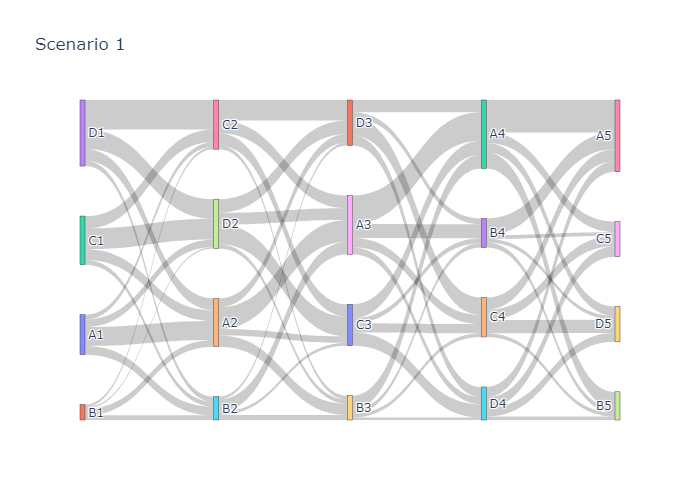
\includegraphics[width=\textwidth]{Figure/Figure26a.jpg}
    \caption{In scenario 1}
    \label{fig26a}
  \end{subfigure}
  \begin{subfigure}{0.5\textwidth}
    \centering
    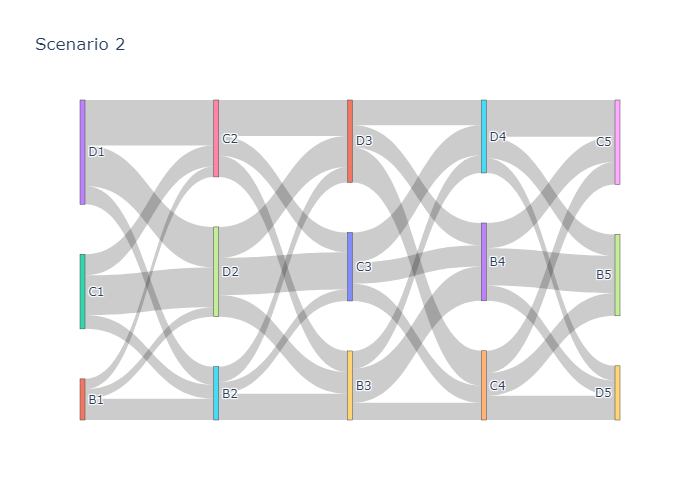
\includegraphics[width=\linewidth]{Figure/Figure26b.jpg}
    \caption{In scenario 2}
    \label{fig26b}
  \end{subfigure}
  \begin{subfigure}{0.5\textwidth}
    \centering
    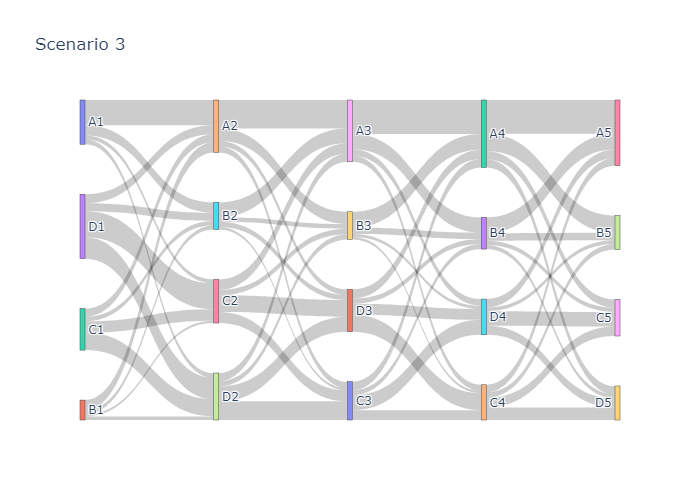
\includegraphics[width=\linewidth]{Figure/Figure26c.jpg}
    \caption{In scenario 3}
    \label{fig26c}
  \end{subfigure}
  \begin{subfigure}{0.5\textwidth}
    \centering
    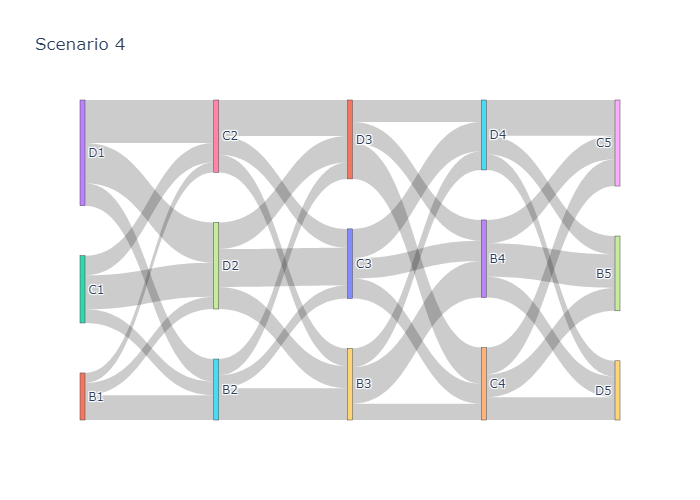
\includegraphics[width=\linewidth]{Figure/Figure26d.jpg}
    \caption{In scenario 4}
    \label{fig26d}
  \end{subfigure}
  \caption{Sankey diagram of foreign visitors }
  \label{fig26}
\end{figure*}

\begin{figure*}[h]
  \begin{subfigure}{0.5\textwidth}
    \centering
    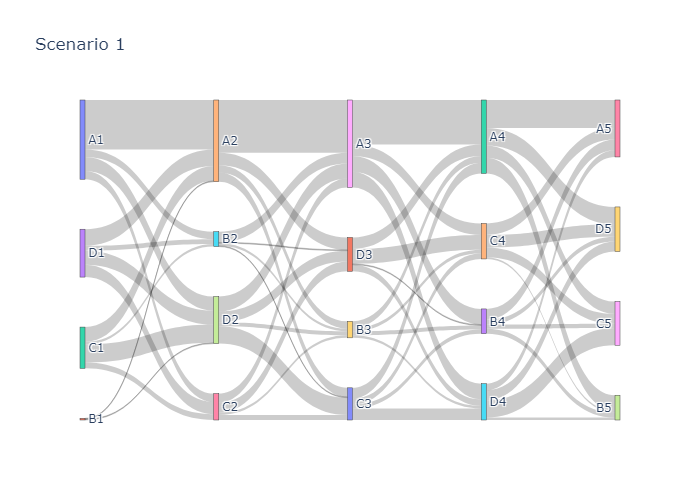
\includegraphics[width=\textwidth]{Figure/Figure27a.jpg}
    \caption{In scenario 1}
    \label{fig27a}
  \end{subfigure}
  \begin{subfigure}{0.5\textwidth}
    \centering
    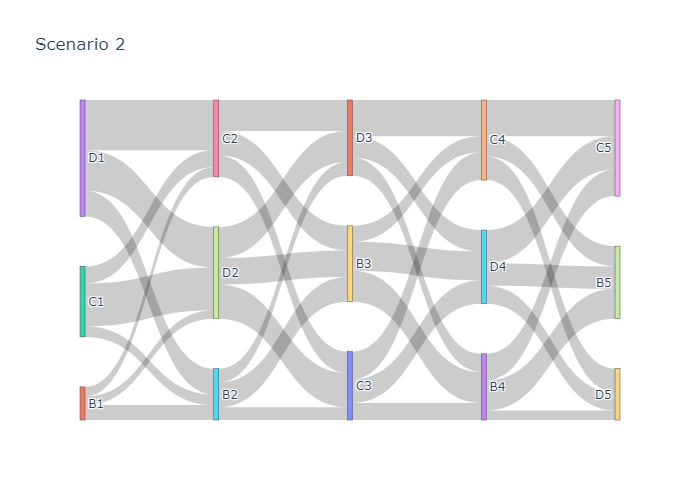
\includegraphics[width=\linewidth]{Figure/Figure27b.jpg}
    \caption{In scenario 2}
    \label{fig27b}
  \end{subfigure}
  \begin{subfigure}{0.5\textwidth}
    \centering
    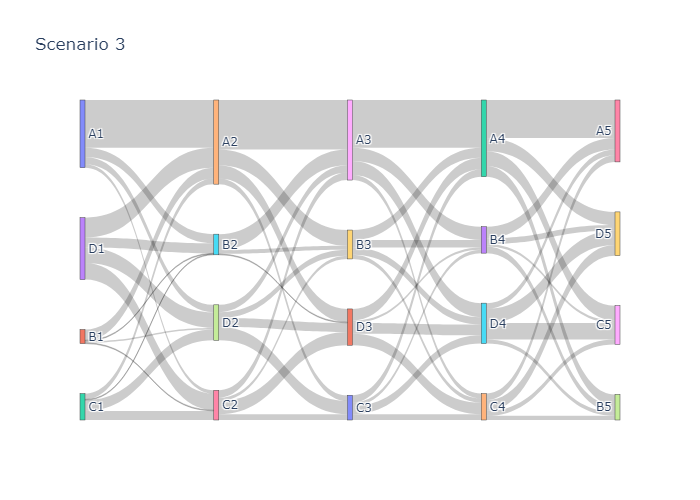
\includegraphics[width=\linewidth]{Figure/Figure27c.jpg}
    \caption{In scenario 3}
    \label{fig27c}
  \end{subfigure}
  \begin{subfigure}{0.5\textwidth}
    \centering
    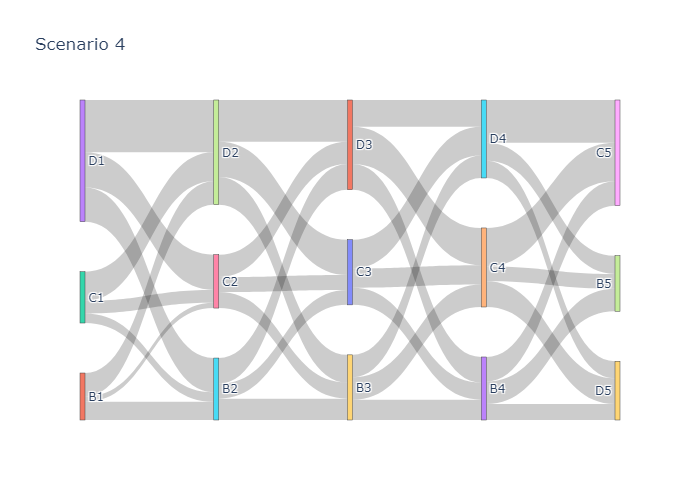
\includegraphics[width=\linewidth]{Figure/Figure27d.jpg}
    \caption{In scenario 4}
    \label{fig27d}
  \end{subfigure}
  \caption{Sankey diagram of Japanese }
  \label{fig27}
\end{figure*}

\begin{figure*}[h]
  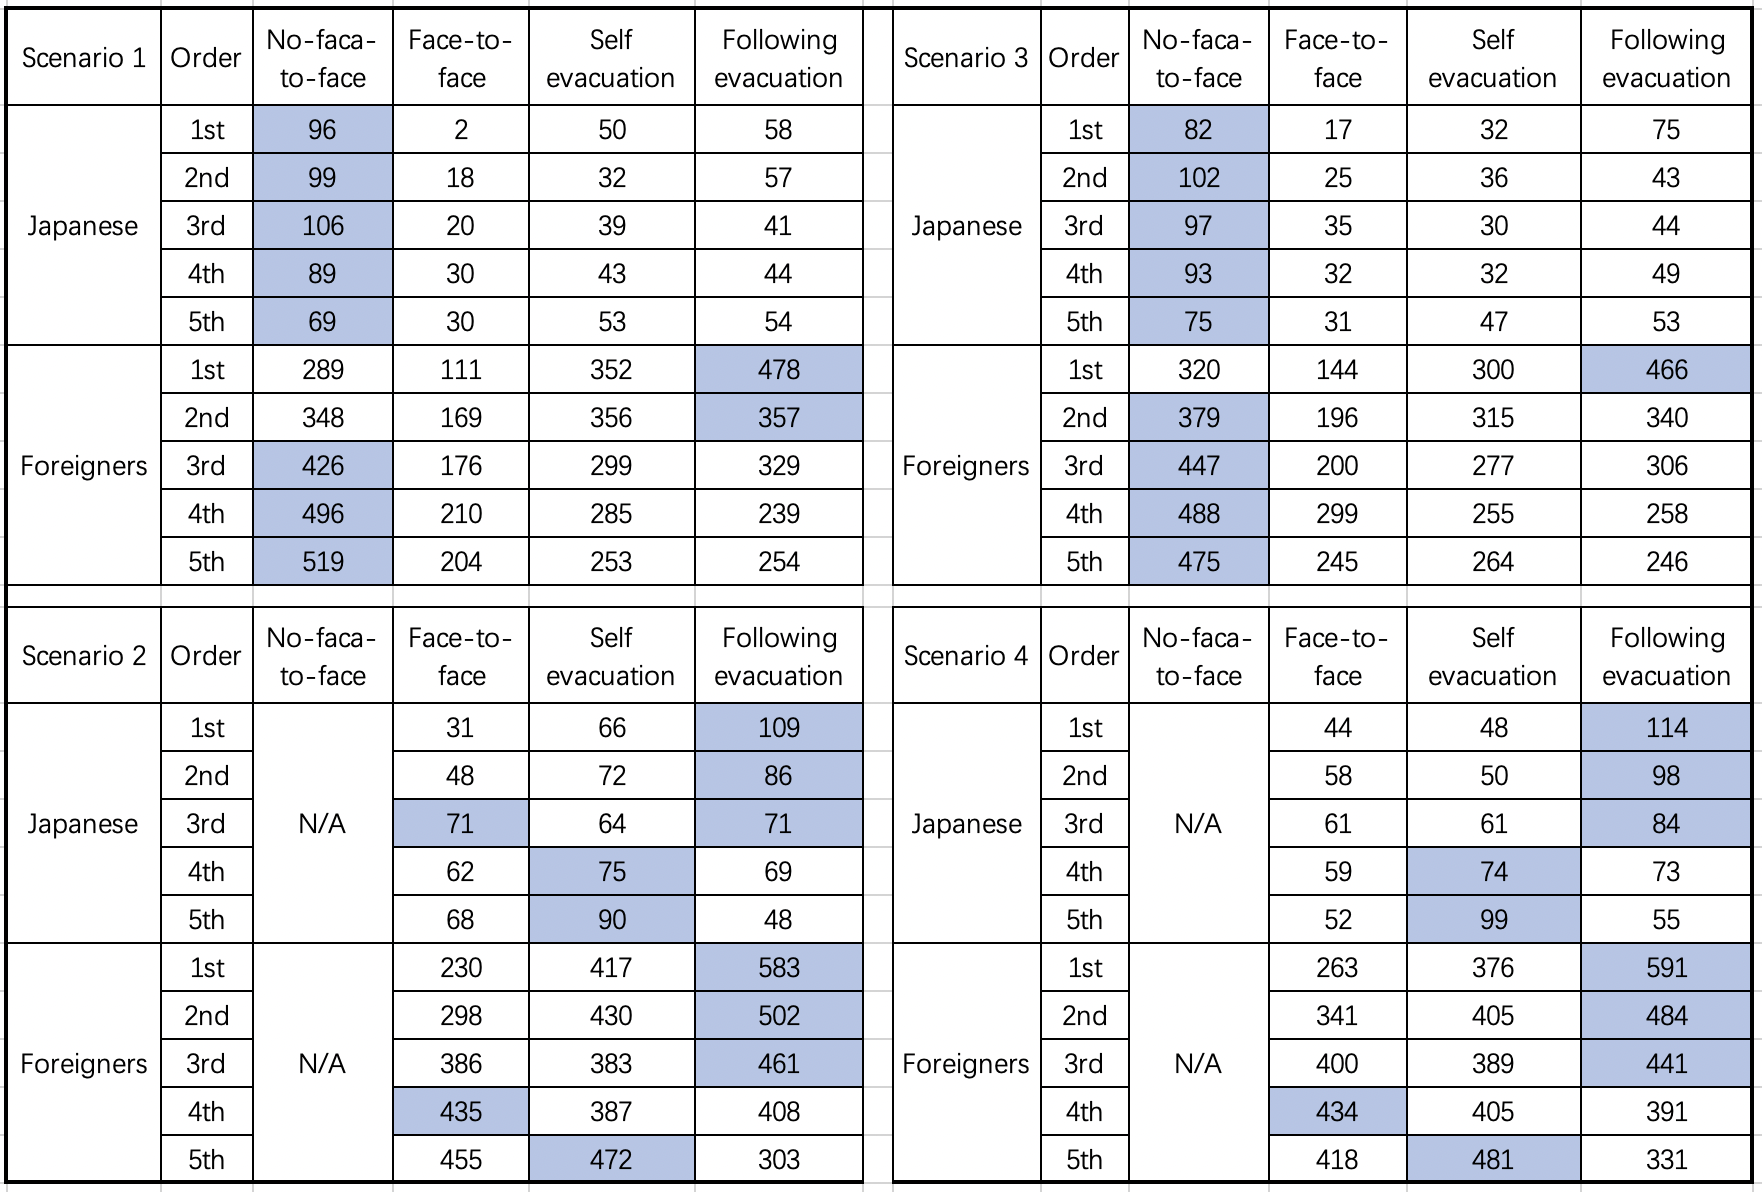
\includegraphics[width=\linewidth]{Figure/Figure28.jpg}
  \centering
  \caption{Summary of Sankey diagram data}
  \label{fig28}
\end{figure*}
%\fi







